\documentclass[12pt,a4paper]{book}
\usepackage[utf8]{inputenc}
\usepackage{ucs}
% \usepackage{pdflscape}
\usepackage{amsmath}
\usepackage{amsfonts}
\usepackage[french]{babel}
\usepackage{amssymb}
\usepackage{glossaries}
\usepackage[bookmarks]{hyperref}
\usepackage{graphics}
\usepackage[pdftex]{graphicx}
\usepackage{latexsym}
\usepackage{cclicenses}

\usepackage{listings}
\usepackage{color}
\usepackage[table]{xcolor}
\definecolor{grey}{RGB}{22,22,22}

\definecolor{mygreen}{rgb}{0,0.6,0}
\definecolor{mygray}{rgb}{0.5,0.5,0.5}
\definecolor{mymauve}{rgb}{0.58,0,0.82}

\usepackage{graphicx}
\lstset{ % general style for listings
   numbers=left
   , tabsize=2
   , frame=single
   , breaklines=true
   , basicstyle=\ttfamily
   , numberstyle=\tiny\ttfamily
   , framexleftmargin=7mm
   , identifierstyle=\color{purple}
   , commentstyle=\color{gray}
   , stringstyle=\color{green!40!black}
   , keywordstyle=\color{orange}
   , xleftmargin=12mm
   , captionpos=b
}

\lstdefinestyle{xslt}
{
    emph={xsl,template,variable,param,for,each,apply,templates,with,param}
    , emphstyle=\color{magenta}
    , emph={[2]match, select, name, mode}
    , emphstyle={[2]\color{cyan}}
}
\usepackage[final]{pdfpages} 
\usepackage{pstricks}
\usepackage{sectsty}
\usepackage[cc]{titlepic}

\usepackage{hyperref,cleveref}

\addto\extrasfrench{%
  \crefformat{table}{#2tableau~#1#3}
  \crefformat{equation}{#2(#1)#3}
  \crefformat{figure}{#2figure~#1#3}
  \crefmultiformat{equation}{#2(#1)#3}%
    { et~#2(#1)#3}{, #2(#1)#3}{ et~#2(#1)#3}
  %
  \def\corollaryautorefname{corollaire}
  \def\definitionautorefname{définition}
  \def\figureautorefname{figure}
  \def\propositionautorefname{proposition}
  \def\subfigureautorefname{figure}
  \def\tableautorefname{tableau}
  %\renewcommand{\subsectionautorefname}{section}
  %\renewcommand{\subsubsectionautorefname}{section}
}

\usepackage[section]{placeins}

\usepackage{tikz}
\usepackage[babel=true,kerning=true]{microtype}

\usetikzlibrary{%
  arrows,%
  calc,%
  shapes.geometric,%
  shapes.misc,%
  shapes.symbols,%
  shapes.arrows,%
  automata,%
  through,%
  positioning,%
  scopes,%
  decorations.shapes,%
  decorations.text,%
  decorations.pathmorphing,%
  shadows}

\makeglossaries

\definecolor{gray}{rgb}{0.4,0.4,0.4}
\definecolor{darkblue}{rgb}{0.0,0.0,0.6}
\definecolor{cyan}{rgb}{0.0,0.6,0.6}

\lstset{
  basicstyle=\ttfamily,
  columns=fullflexible,
  showstringspaces=false,
  commentstyle=\color{gray}\upshape
}

\usepackage{geometry}
\usepackage{caption}
\geometry{hmargin=2.5cm,vmargin=2.5cm}
\author{Jaussoin Timothée - Polytech Nantes\\ Année 2013--2014 \\
\\ \\ Inspire -- Utrecht -- Pays-Bas\\  Maitre de Stage Floris Vlasveld\\ Enseignant Responsable Normand Nicolas}
\title{Développement Web sur le framework Ruby on Rails}
\titlepic{\begin{center}
	\begin{tabular}{ll}
		
\includegraphics[width=0.3\textwidth]{img/logo.png} \\
		
\includegraphics[width=0.3\textwidth]{img/polytech.jpg} \\ 
	\end{tabular}
\end{center}}
\begin{document}

\begin{titlepage}
	\maketitle
\end{titlepage}

\tableofcontents

\newpage
\clearpage
\vspace*{\stretch{1}}
    \section*{Résumé}
	%Wirelab Creative est une jeune start-up se spécialisant dans le développement de sites web promotionnels localisée à Enschede aux Pays-Bas.
	
	%L'objectif de ces quatre mois de stage a été de maitriser les différentes méthodes de travail de l'équipe ainsi que les technologies web utilisées pour le développement de leurs projets.

  Inspire est une entreprise se spécialisant dans le développement de sites web en utilisant le framework Ruby on Rails. Elle est localisée à Utrecht aux Pays-Bas.
  
  L'objectif de ces six mois de stage a été de conforter les connaissances acquises l'été dernier concernant ce framework ainsi que les différentes technologies liées à l'environnement Web tel que Javascript, CSS ou HTML.

    Ce présent rapport détaillera ces différentes tâches et sera accompagné d'un retour personnel pour chacune.  
\vspace*{\stretch{1}}

\newpage
\clearpage
\vspace*{\stretch{1}}
\section*{Remerciements}

Je tiens à remercier M. Floris Vlasveld, mon maître de stage, ainsi que l'ensemble de l'équipe pour m'avoir accueilli au sein de leurs locaux et pour avoir permis le bon déroulement de mon stage.

%Je remercie également mes collègues Romain Jacob (expert JAVA), Nicolas Ocquidant (expert JAVA), Michael Tallet (architecte logiciel), 
%Sébastien Coché (architecte infrastructure), Julien Pariat (architecte infrastructure), Pascal Pineau (architecte logiciel), Benoit Courtel (ingénieur méthodes de développements) qui m'ont été très utiles tant dans leurs conseil et avis que pour mon intégration au sein de l'équipe.

%<Remercier personnellement>

Enfin, je remercie également M. Nicolas Normand, professeur à Polytech Nantes qui a également veillé au bon déroulement de mon stage.

\vspace*{\stretch{1}}

\chapter{Inspire}

L'entreprise Inspire, localisée à Utrecht, se spécialise depuis 2011 dans la conception d'applications web sur la technologie Ruby on Rails. Dans ce chapitre nous détaillerons l'historique de l'entreprise afin de mieux comprendre son status actuel.

\section{Historique}
\subsection{2011 - Création de Inspire}

Mr Vlasveld Floris fonda Inspire fin 2011 afin d'avoir une structure légale pour le lancement d'un projet avec The Dutch Cancer Society\footnote{\url{http://www.kwf.nl/}} suite à un appel d'offres. Ce projet devant se dérouler sur un mois il recrute alors deux freelancers afin de travailler sur l'élaboration de la plateforme sur le framework Ruby on Rails.

Plusieures technologies ont été envisagées jusqu'alors mais c'est Rails qui a finalement été retenu. Ce choix constituera une orientation décisive dans la technologie mère que Inspire souhaite utiliser au sein de son équipe au fil des années.

\subsection{2012 - Elsevier, développement}

Début 2012, Inpire commence à travailler sur un second projet. Le but est alors de développer un puissant outil de visualisation de statistiques de publications pour l'éditeur Elsevier\footnote{\url{http://www.elsevier.com/}}, numéro un mondial dans la publication de revues scientifiques (comprenant pas moins de 1800 références dans son catalogues).

La plateforme permet également aux auteurs de sélectionner intelligement la revue la plus pertinente dans laquelle ils seront publiés.

Parallèlement à ce projet, le partenariat avec KWF sera renforcé via un rapprochement des deux structures pour un travail futur sur d'importants projets.

Suite à cette demande Mr Vlasveld décide de recruter plusieurs freelancers courant avril afin de renforcer son équipe de développeurs.

En mai l'équipe commence à travailler sur le projet remporté fin 2011 avec KWF, au sein de leurs locaux. Cette importante application occupera l'équipe jusqu'à la fin de l'année et monopolisera jusqu'à 9 développeurs en freelance.

\subsection{2013 \& 2014 - Équipe et locaux}

L'année 2013 marquera le début de l'indépendance de Inspire vis à vis de KWF, le projet alors développé continuera d'être géré en interne par un nouveau Scrum Master (Mr Vlasveld occupant jusqu'alors cette position).

Courant février Mr Vlasveld recrute ses premiers employés à temps plein puis commence à constituer une équipe de 4 développeurs qui travaillerons de façon continue sur les projets importants.

Au début de l'année 2014 l'équipe eménage dans de nouveaux locaux dans le nord de Utrecht.

De nombreux projets sont alors acceptés et l'équipe se stabilise sur sa structure (cinq membres dont deux développeurs ``frontend'' et deux développeurs ``backend''). Courant février 2014 un manager de projets est recrutée pour épauler Mr Vlasveld et ainsi lui permettre se se concentrer sur ses tâches principales : la relation client et la gestion générale de l'agence.

J'ai rejoint l'équipe peu avant le recrutement du nouveau manager de projets.

\section{L'Équipe}

L'équipe de Inspire est particulièrement resserée et est composée de quatres développeurs et de deux managers. Le fait de concentrer les technologies exploitées au sein d'Inspire autour du framework Ruby on Rails permet aux développeurs de monter en compétences sur certains points particuliers de cet environnement plutôt que sur de multiples outils et frameworks.

Quelques autres personnes, travailleurs indépendants, sont également liés à l'équipe et participent ponctuellement sur des projets.

Cette organisation permet à Inspire de travailler avec une équipe dynamique et pouvant s'adapter à toutes les situations. Par exemple, durant des moment difficiles, il n'est pas rare que une ou deux personnes viennent renforcer l'effectif pour fluidifier le travail et sa répartion. 

Il est aussi intéressant de noter que chaque développeur possède des abilités particulières sur certains des aspects du développement des applications web. Certains par exemple ont plutôt tendance à travailler sur l'interface avec l'utilisateur (on parle alors de développeurs ``frontends'') tandis que d'autres apprécient le développement de l'architecture coté serveur (ils sont alors vu comme des développeurs ``backend'').

\subsection{Organigramme}

Vous pouvez retrouvez l'organigrame \cref{fig:1}. Mon poste pouvant être ici placé au même niveau que les autres dévelopeurs.


\begin{figure}[h]
   \centering
\begin{tikzpicture}
\begin{scope}[xscale=2,yscale=1.5]
% description et nommage des noeuds 
\node (D) at (0,4) [rectangle,draw] {\begin{tabular}{c}\textbf{Directeur}\\Floris Vlasveld\end{tabular}};
\node (PM) at (2,2.8) [rectangle,draw] {\begin{tabular}{c}\textbf{Project Manager}\\Anne-Lot Rameau\end{tabular}};
\node (D1) at (-3,1) [rectangle,draw] {\begin{tabular}{c}\textbf{Developer}\\David Boot\end{tabular}};
\node (D2) at (-1,1) [rectangle,draw] {\begin{tabular}{c}\textbf{Developer}\\Joshua Jansen\end{tabular}};
\node (D3) at (1,1) [rectangle,draw] {\begin{tabular}{c}\textbf{Developer}\\Martina Šimičić\end{tabular}};
\node (D4) at (3,1) [rectangle,draw] {\begin{tabular}{c}\textbf{Developer}\\Garm Lucassen\end{tabular}};
\draw (0,2) -- (D);
\draw (0,2.8) -- (PM);
\draw (0,2) -| (D1);
\draw (0,2) -| (D2);
\draw (0,2) -| (D3);
\draw (0,2) -| (D4);
\end{scope}
\end{tikzpicture}
\caption{\label {}Organigramme de l'équipe fixe de Inspire} 
\label{fig:1}
\end{figure}

\subsection{Mon rôle dans l'équipe}

Mon intégration s'est faite en plusieurs étapes. J'ai tout d'abord passé quelques semaines à comprendre le fonctionnement de l'équipe et du projet Calibris (voir \cref{sec:calibris}) via la lecture de son code source et la réorganisation de quelques fichiers.

Ayant déjà les bases nécessaires à la bonne compréhension d'un projet Ruby on Rails standard (en grande partie grâce au stange que j'avais déjà fait l'année dernière) la majeure partie des informations que je devais assimiler se portaient sur les algorithmes et spécificités de ce projet (étapes de validation des formulaires, limitations mais aussi structure générale des modèles gérés par l'application).

Durant ce stage j'ai eu la possibilité de m'améliorer sur plusieurs aspects très distincs.

\subsubsection{Organisationel}

D'un point de vue organisationel j'ai eu la possibilité de m'exprimer sur quelques points relatifs aux projets d'Inspire. J'ai par exemple organisé plusieurs réunions avec mes collègues afin de les informer de difficultés actuelles ou futures du projet Calibris pour que nous prenions ensemble une décision pour les corriger.

La structure organisationnelle d'Inspire, s'articulant sur de nombreux aspects sur les méthodes Agiles encourage également une forte cohésion entre les membres de l'équipe avec des échanges quotidients.

J'ai donc pu avoir de très nombreuses occasions de m'exprimer au sein de l'équipe afin de proposer des idées d'amélioration tant sur le plan technique que relationel.

\subsubsection{Technique}

Sur le plan technique j'ai amené certaines connaissances concernant le développement Web grâce aux expériences et problèmes que j'ai pu avoir auparavant sur les nombreux projets que j'ai fais parallèlement à mes études. J'ai notamment apporté de mon aide sur des problèmes relatifs à l'optimisation de l'éxécution du Javascript au sein du navigateur et à son utilisation en liaison avec l'arbre structurel de la page (plus communément appelé arbre DOM\footnote{Le Document Object Model (ou DOM) est un standard du W3C qui décrit une interface indépendante de tout langage de programmation et de toute plate-forme, permettant à des programmes informatiques et à des scripts d'accéder ou de mettre à jour le contenu, la structure ou le style de documents XML et HTML. Le document peut ensuite être traité et les résultats de ces traitements peuvent être réincorporés dans le document tel qu'il sera présenté.. Source \url{http://fr.wikipedia.org/wiki/Document_Object_Model}}).

J'ai également apporté de mon aide aux autres développeurs en leurs offrant une vision extérieure aux problèmes qu'ils avaient, ici encore particulièrement vis à vis des soucis relatifs au Javascript, HTML et CSS. 

\subsubsection{Humain}

Pour le coté humain j'ai également donné de ma personne afin de participer à la bonne vie de l'équipe. Je pense que ce point est sûrement l'un des plus important que j'ai eu à exprimer au sein de mon stage, également grâce à l'utilisation des méthodes Agiles. Je le développerai dans la dernière partie de ce rapport.

\chapter{Notions préalables}

Dans ce chapitre je détaillerai un ensemble d'éléments techniques nécessaires à la bonne compréhension du reste du rapport. Je présenterai également les méthodes de développement et techniques utilisées au sein de l'agence pour leurs projets.

\section{Ruby on Rails}

L'ensemble des projets gérées au sein de Inspire sont écrits grâce à l'utilisation du framework Ruby on Rails.

Le framework Ruby on Rails rassemble énormément de concepts et technologies déjà largement présents dans le domaine du développement d'applications : Model-Vue-Controlleur\footnote{Le patron modèle-vue-contrôleur (en abrégé MVC, de l'anglais model-view-controller), tout comme les patrons modèle-vue-présentation ou Présentation, abstraction, contrôle, est un modèle destiné à répondre aux besoins des applications interactives en séparant les problématiques liées aux différents composants au sein de leur architecture respective. Source \url{http://fr.wikipedia.org/wiki/Modele-Vue-Controleur}}, REST\footnote{REST (REpresentational State Transfer) est un style d’architecture pour les systèmes hypermédia distribués, créé par Roy Fielding en 2000 dans le chapitre 5 de sa thèse de doctorat. Source \url{http://fr.wikipedia.org/wiki/Rest}}, JSON\footnote{JSON (JavaScript Object Notation) est un format de données textuelles, générique, dérivé de la notation des objets du langage ECMAScript. Il permet de représenter de l’information structurée. Créé par Douglas Crockford, il est décrit par la RFC 4627 de l’IETF. Source \url{http://fr.wikipedia.org/wiki/Json}} ou encore le Mapping objet-relationnel\footnote{Un mapping objet-relationnel (en anglais object-relational mapping ou ORM) est une technique de programmation informatique qui crée l'illusion d'une base de données orientée objet à partir d'une base de données relationnelle en définissant des correspondances entre cette base de données et les objets du langage utilisé. On pourrait le désigner par « correspondance entre monde objet et monde relationnel » . Source \url{http://fr.wikipedia.org/wiki/Mapping_objet-relationnel}}.

L'utilisation exclusive de ce framework permet à l'ensemble des membres d'Inspire de ne se concentrer que sur un seul outil. En effet il est courant de rencontrer des agences qui travaillent simultanément sur plusieurs frameworks et CMS\footnote{Un système de gestion de contenu ou SGC (Content Management System ou CMS) est une famille de logiciels destinés à la conception et à la mise à jour dynamique de sites Web ou d'applications multimédia. Source \url{http://fr.wikipedia.org/wiki/Systeme_de_gestion_de_contenu}} et celà au sein d'une équipe de quelques personnes uniquement.

Mais bien au delà des capacités fonctionnelles offertes par Ruby on Rails, c'est toute la méthodologie liée à l'utilisation du framework qui est ici intéressante à exploiter. En effet celui-ci offre de très nombreux outils et conventions permettant aux développeurs de structurer leur travail et d'éviter de redévelopper des choses pré-existantes. De nombreux mécanismes de contrôles permettent également d'alerter l'équipe en cas d'apparition d'erreurs pendant le développement (nous détaillerons cet élément un peu plus tard) mais aussi de fournir des indices de performance détaillés facilitant grandement l'optimisation et l'amélioration générale du fonctionnement de l'application.

\subsection{Les Gems}

La construction d'une application Ruby on Rails passe avant tout par l'intégration d'un ensemble de modules appelés \textit{gems} au sein du projet. Ceux-ci ont comme rôle d'intégrer de nouvelles fonctionnalités ou de permettre certaines actions particulières sans avoir à redévelopper l'outil. 

La liste de ces modules est à déclarer dans le fichier \texttt{Gemfile} disponible à la racine du projet.

C'est l'outil \texttt{bundle} qui récupérera les archives depuis le dépot RubyGems\footnote{\url{http://rubygems.org/}} et déploiera les \textit{gems} lors de la récupération de l'application. Un numéro de version peut également être spécifié à la suite du nom afin de figer l'environnement de déploiement et ainsi éviter toute incompatibilité future lors de la mise à jour des modules.

\begin{figure}[h]
\lstset{language=ruby}
\begin{lstlisting}
source 'https://rubygems.org'

gem "rails", "~>3.2.17"

gem "ansi", "~>1.4", :require => nil
gem "acts_as_list", "~>0.1.6"
gem "bitfields", "~>0.4"
...
\end{lstlisting}
 \caption{Extrait d'un fichier \texttt{Gemfile}}
\end{figure}

\subsection{Les environnements}

Dans une application RoR, les différentes étapes du développement son intégrées au sein de l'application. De ce fait, lors de l'intégration d'une nouvelle fonctionnalité dans le code source plusieurs étapes seront à passer avant de pouvoir déployer le nouveau code source en production.

Nous retrouvons principalement trois environnements :
\begin{description}
	\item[development] étape concernant l'intégration des nouveaux composants dans le code source
	\item[test] étape s'occupant de tester les nouvelles fonctionnalités et de vérifier si aucune régression n'est apparue 
	\item[production] étape où l'application se retrouve dans son environnement final
\end{description}
Nous pouvons également remarquer que chaque environnement possède sa propre base de donnée afin de séparer hermétiquement les données des différentes étapes. 

\subsection{Les tests}

\label{sec.tests}

Tout élément développé au sein de Ruby on Rails peut faire l'objet d'un test afin de vérifier son bon déroulement. Au sein de Inspire deux types de tests sont écrits.

\subsubsection{RSpec}

RSpec est un \textit{gem} permettant l'écriture de tests unitaires\footnote{En programmation informatique, le test unitaire est une procédure permettant de vérifier le bon fonctionnement d'une partie précise d'un logiciel ou d'une portion d'un programme (appelée « unité » ou « module »).\url{http://fr.wikipedia.org/wiki/Tests_unitaires}} sur les trois parties du MVC dans une application RoR.
\begin{description}
	\item[Modèles] Les modèles peuvent être testés en vérifiant, entre autre, la bonne affectation des valeurs des attributs, le respect des contraintes qui ont été définies (par exemple nous pouvons vérifier qu'une variable n'est pas enregistrée en base de donnée si celle-ci dépasse une valeur maximale définie).
	\item[Controlleurs] Nous pouvons tester les contrôleurs en vérifiant les valeurs retournées et les comportements définits en leur sein (par exemple si une redirection de page est bien exécutée à la fin d'une étape).
	\item[Vues] Les vues sont testés en vérifiant la présence (ou non) de certains éléments lors de l'affichage de la page. 
\end{description}

\begin{figure}[h]
\lstset{language=ruby}
\begin{lstlisting}
require 'spec_helper'

describe DiariesController do
  let(:diary) { FactoryGirl.create(:diary) }
  let(:owner) { diary.owner }

  it "shows the diary" do
    get :show, user_id: owner, id: diary
    response.should be_success
  end

  context "Deleted diary" do
    before(:each) { diary.mark_as_deleted }

    it "doesn't show the deleted diary" do
      get :show, user_id: owner, id: diary
      response.should contain('Acces interdit a cette page !')
    end
  end
end
\end{lstlisting}
 \caption{Test unitaire d'un contrôleur}
\end{figure}

Au sein de ce test nous pouvons apercevoir différentes chôses. Tout d'abord le \textit{gem} RSpec vient avec une syntaxe qui lui est propre. Celle-ci s'articule particulièrement autour des mots clefs \texttt{describe}, \texttt{context} et \texttt{it}. Le mot clef \texttt{it} permettant de décrire un test à proprement parler et doit toujours être contenu dans un \texttt{describe}. Le mot clef \texttt{context} quant-à lui permet de regrouper les tests par catégories afin d'en simplifier l'organisation, la lecture et le débuggage.

Un test RSpec s'effectue toujours en deux temps :
\begin{description}
	\item[Le contexte] d'exécution dans lequel nous allons définir dans quel état sera l'application au moment de l'exécution du test. Dans notre cas nous créons préalablement une instance \texttt{diary} depuis la base de donnée. Puis nous tentons de charger la page pour afficher cette instance via l'appel de la méthode \texttt{get} qui va simuler un chargement virtuel.
	\item[L'épreuve], une fois le contexte définit le test consistera a vérifier si un ou des éléments de l'environnement est dans l'état où il devrait être. Ici nous vérifions si le chargement de la page demandée est fructueuse (et si elle contient un certain texte pour le second test).
\end{description}

Chaque test sera exécuté indépendament des autres (en particulier vis à vis des instances pré-chargées en mémoire) et celà afin d'éviter tout comportement non voulu de l'application ce qui pourrait résulter d'un faux positif.

\subsubsection{Cucumber}

Cucumber\footnote{\url{https://github.com/cucumber/cucumber-rails}} est également un \textit{gem} permettant l'écriture de tests. Mais contrairement à RSpec celui-ci se situe à un plus haut niveau en décrivant le comportement des utilisateurs via l'interface. Ces tests sont directement écrits à partir des scénarios utilisateurs approuvés par le client.

Deux niveaux d'abstraction existent lors de la rédaction des tests Cucumber. Le développeur va tout d'abord rédiger en anglais un ensemble d'étapes qui devront être effectuées pour la validation du test.

\begin{figure}[h]
\lstset{language=ruby}
\begin{lstlisting}
Feature: Manage Categories
  As an Admin I want to be able to manage Questions in a Questionnaire

  Background:
    Given I have created an "Admin" and I am signed in
    Given There is a Cluster

  Scenario: I create a Question
    Given I visit the Questionnaire page
    And I click new Question
    Then I see the new Question form
    And I fill out a label
    And I submit the form
    Then I see the Question on the Questionnaire page
\end{lstlisting}
 \caption{Test Cucumber sur la création d'une Question}
\end{figure}

Ici nous voyons parfaitement que la rédaction d'un ensemble de tests peut être fait par l'interprétation des scénarios utilisateurs validés avec le client. Il est d'ailleur conseillé d'effectuer cette tâche avec le principal intéressé afin d'être sûr que les fonctionnalités qui seront développées suite à ces tests coïncident bien avec les attentes de celui-ci.

Par la suite le développeur aura comme tâche d'écrire les actions exécutées pendant les différentes étapes afin de dicter au simulateurs quoi faire pour chacunes d'entre elles.

\begin{figure}[h]
\lstset{language=ruby}
\begin{lstlisting}
Given(/^I click new Question$/) do
  click_link I18n.t('questions.create.title')
end

Then(/^I see the new Question form$/) do
  page.should have_content I18n.t('questions.create.title')
  page.should have_content @questionnaire.name
end

Then(/^I fill out a label$/) do
  fill_in :question_label, with: "Question label"
end

Then(/^I see the Question on the Questionnaire page$/) do
  visit questionnaire_path(@questionnaire)
  page.should have_content "Question label"
end
\end{lstlisting}
 \caption{Définitions des différentes étapes de tests Cucumber}
 \label{fig.cucumber2}
\end{figure}

Cucumber travaille étroitement avec un autre projet nommé Capybara\footnote{\url{https://github.com/jnicklas/capybara}} qui fera office de simulateur lors de l'exécution des tests. Certaines des directives écrites dans la \cref{fig.cucumber2} dictent à Capybara quelle action effectuer (tel que \texttt{visit}, \texttt{fill\_in}\dots). Suite à ça des vérifications peuvent êtres faites afin de valider le bon déroulement des actions. 

Ces vérifications passent par l'appel de méthodes qui vérifierons si la page résultante possède le contenu attendu (ou non) ou si certaines variables englobant l'exécution de la page (tel que les variables de session ou les variables \texttt{GET} et \texttt{POST} envoyées par le navigateur) possèdent les bonnes valeurs.

Nous pouvons également notter que ces étapes peuvent être parfaitement réutilisées entre les tests pour éviter toute redondance de code.

\subsubsection{En bref}

Les deux types de tests intégrés aux applications à Inspire permettent de couvrir efficacement la majeur partie des éléments développés. Ceux-ci sont systématiquement (et de façon automatique) exécuté lors de la publication de nouveaux codes sources sur les dépots Git.

Des outils tel que CodeShip\footnote{\url{https://www.codeship.io/}} ou CircleCi\footnote{\url{https://circleci.com/}} permettent d'effectuer ces tests sur des fermes de calcul et d'en afficher les résultats sur les branches sur lesquelles travaillent les développeurs afin de les notifiers de toute régression. L'ensemble de ces techniques font partie du concept plus général d'intégration continue activement pratiquée à Inspire.

\section{Gestion de projet}

Avant d'entre de façon concrète au sein des différents projets dans lesquels j'ai pris part il est également intéréssant de décrire et de comprendre les méthodes de travails pratiquées au sein de Inspire.

\subsection{Omniprésence des méthodes Agiles}

Les méthodes Agiles sont courrament utilisées à Inspire. La taille des projets amenant l'équipe à travailler par cycles (ou Sprints) de deux semaines. Une réunion appellée ``daily standup'' est également organisée tous les matins afin que chaque membre puisse mettre au courant le reste de l'équipe de ses avancées sur les tâches qui lui sont sont présentement affectées. Cette réunion est également l'occasion de présenter les tâches qui seront traitées pendant la journée.

\begin{figure}[htp]
\centering
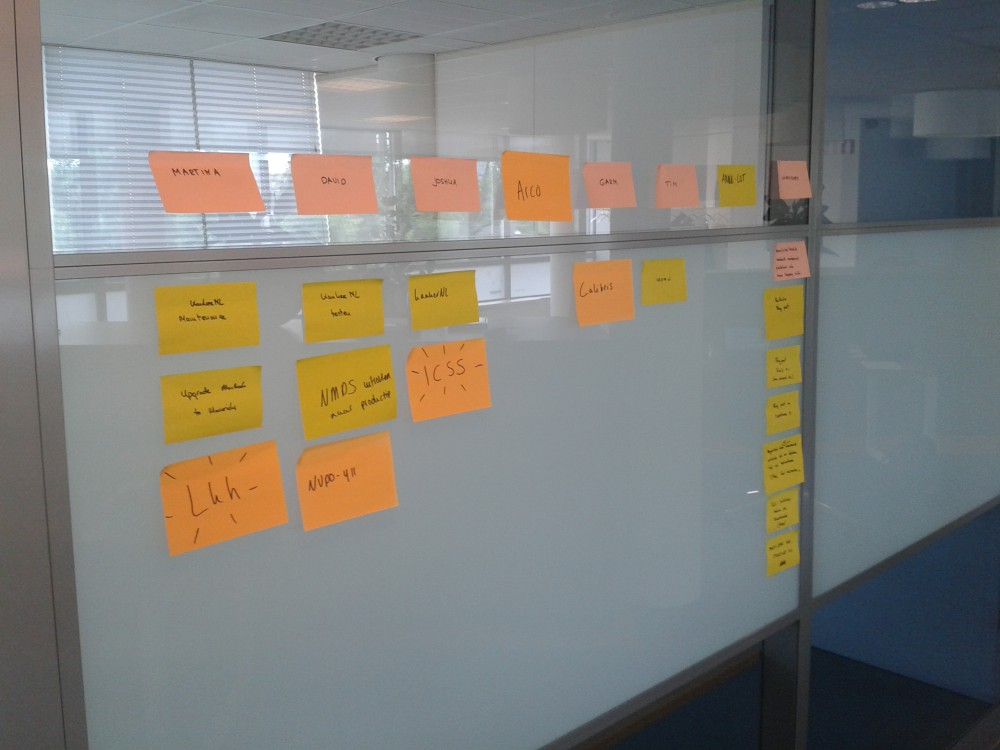
\includegraphics[scale=.40]{img/agile1.jpg}
 \caption{Le ``Scrum Board'' permettant d'avoir une vision globale des tâches}
 \label{fig.agile1}
\end{figure}

Mais au delà des cycles de développement, c'est l'organisation même des projets qui se sont adaptées à ces méthodes. De ce fait, l'ajout de toute nouvelle fonctionnalité dans un projet est jalonnée par un ensemble d'étapes obligatoires pour le bon déroulement et le respect des méthodes d'intégration continues.

\subsubsection{Particularités relatives à Inspire}

L'utilisation des méthodes Agiles au sein d'Inspire diffère sur certains points par rapport à ce que j'ai vécu lors de mon précédent stage (qui s'est fait autour d'un sujet similaire, au sein d'une équipe travaillant également avec certaines méthodes Agiles).

Tout d'abord, comme précisé précédement, l'équipe d'Inspire travaille au sein de cycles allant de deux à trois semaines. Ce rythme est ici plus en phase avec la taille des projets développés. Les fonctionnalités étant importantes elles nécessitent bien souvent plusieurs développeurs à plein temps pour mener leurs développement à terme. 

Il y a également deux tableaux Scrum, l'un virtuel, l'autre affiché dans le bureau. Le tableau virtuel est géré grâce à Jira (voir \cref{sec.jira}) et permet de gérer les tâches de l'ensemble des projets au jour le jour. L'autre offre une vision plus globale (voir \cref{fig.agile1}) et concerne plus la répartition des tâches globales entre les membres de l'équipe.

\subsection{Git et GitHub}

\label{sec.git}

L'intégralité du code source développé est organisé grâce au gestionnaire de code Git. La forge Github\footnote{\url{https://github.com/}} servant de point central pour l'hébergement et la gestion des différentes branches.

Il est ici intéressant de voir la méthodologie que l'équipe a appliqué, grâce aux fonctionnalités offertes par Github, pour gérer le code source écrit par les membres de chaque projets.

En effet, chaque étape ou module sera considéré comme une branche de travail issue de la branche principale (appelée \texttt{master} ou \texttt{trunk}). Lorsqu'un développeur souhaite implémenter une nouvelle fonctionnalité ou réécrire un partie du code source, celui-ci va créer une nouvelle branche (il va ``forker''), effectuer ses modifications puis faire une proposition au reste de l'équipe, cette offre est appelée ``pull request'' (car l'idée est de ``tirer'' les modifications dans la branche d'origine).

\begin{figure}[htp]
\centering
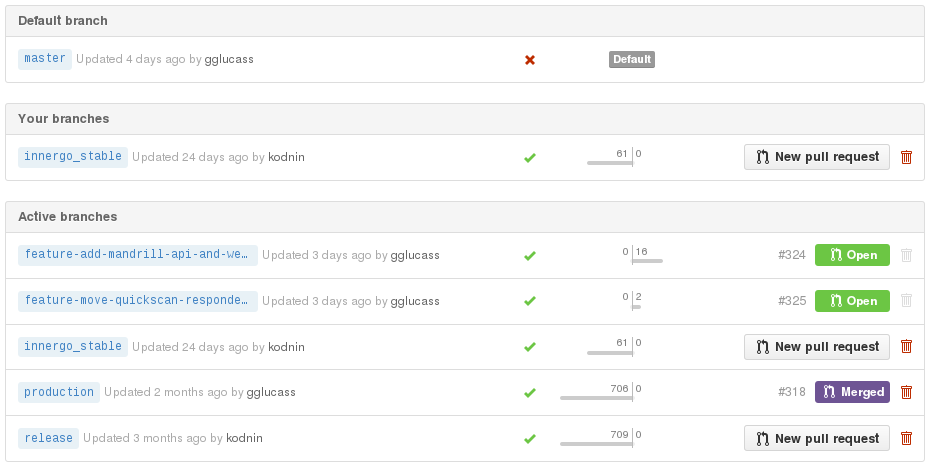
\includegraphics[scale=.50]{img/branches.png}
 \caption{Aperçu du gestionnaire de branches de GitHub pour le projet Calibris}
 \label{fig.jira_agile1}
\end{figure}

Chacune des branches devra par la suite être revue par un collaborateur n'ayant pas participé à la rédaction du code source la contenant, cela permet d'avoir un œil externe sur le code rédigé permetant ainsi de détecter des optimisations, des erreurs ou de simples fautes d'innatentions.

Chaque branche devra également comporter son lot de nouveaux tests (RSpec et Cucumber) afin de couvrir le code nouvellement rédigé (certains outils tel que CodeClimate\footnote{\url{https://codeclimate.com/}} analysent et génèrent automatiquement des rapports précisant la couverture du code source des projets et les points à améliorer).

Après la revue du code source, la rédaction des nouveaux tests et la validation des tests préexistants le développeur est alors autorisé à fusionner (ou ``merger'') son code source avec le code d'origine. La nouvelle fonctionnalité faisant alors partie intégrante du projet.

\subsection{Jira}

\label{sec.jira}

Essentiellement tourné vers la gestion du code source, GitHub n'offre pas l'ensemble des fonctionnalités nécessaires à la bonne gestion et au bon déroulement des projets.

Toute la partie suivit et gestion de projet (notamment la partie Agile) est supervisée par Jira. Celui-ci est composé de nombreux modules s'occupant des différents aspects du développement et de la résolution des tâches au sein de l'entreprise.

Nous retrouvons par exemple un Wiki général servant, entre autre, à la rédaction et au partage d'informations communes concernant l'organisation générale du travail au sein de l'équipe, mais également un gestionnaire de projets qui permet aux développeurs et aux managers d'avoir une vue générale de l'état de chaque projet en cours.

Nous détaillerons ici deux éléments centraux dans l'application, à savoir le module Agile et le Module Tempo.

\subsubsection{Le module Agile}

\begin{figure}[htp]
\centering
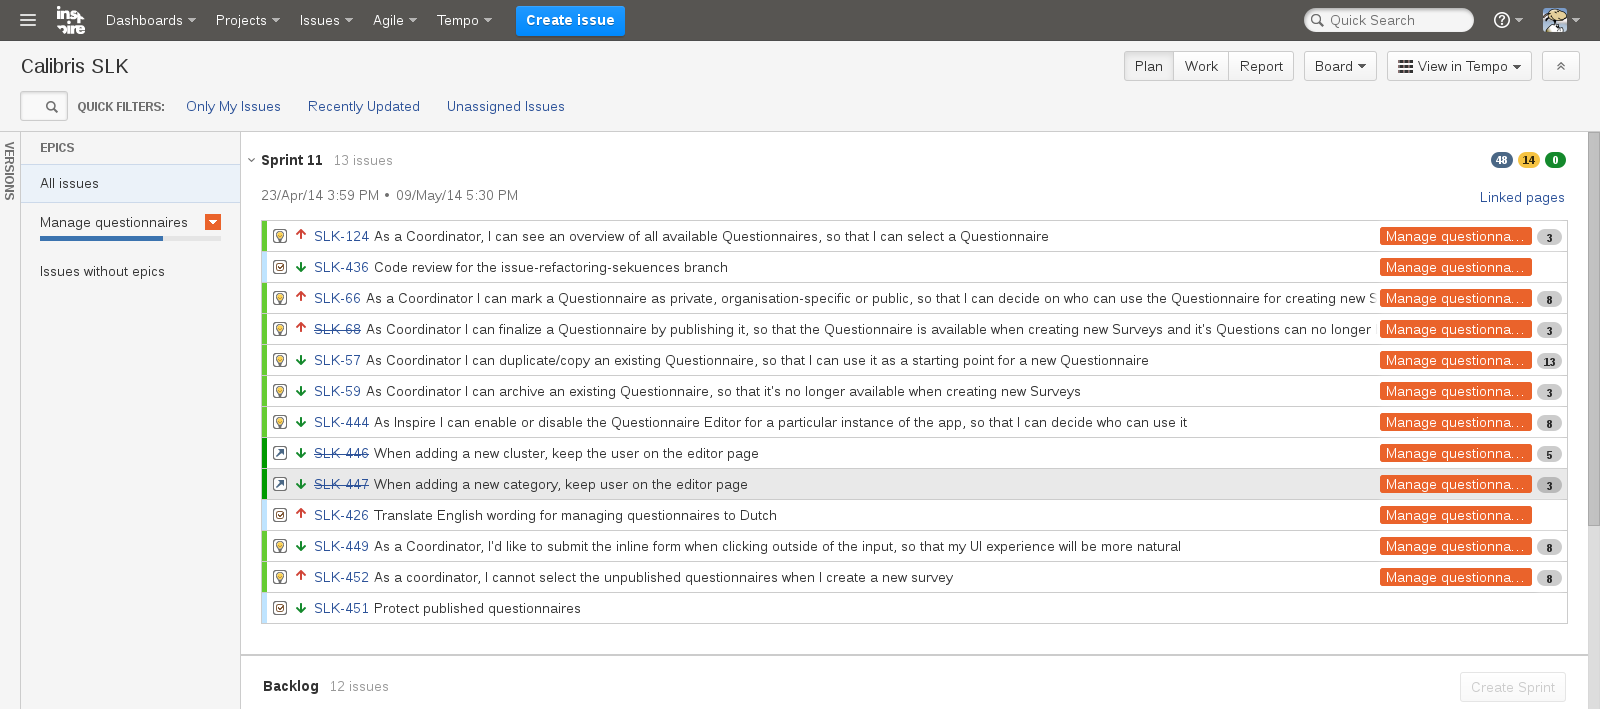
\includegraphics[scale=.30]{img/jira_agile_1.png}
 \caption{Vue des tâches du projet en cours sur le module Agile de Jira}
 \label{fig.jira_agile1}
\end{figure}

\begin{figure}[htp]
\centering
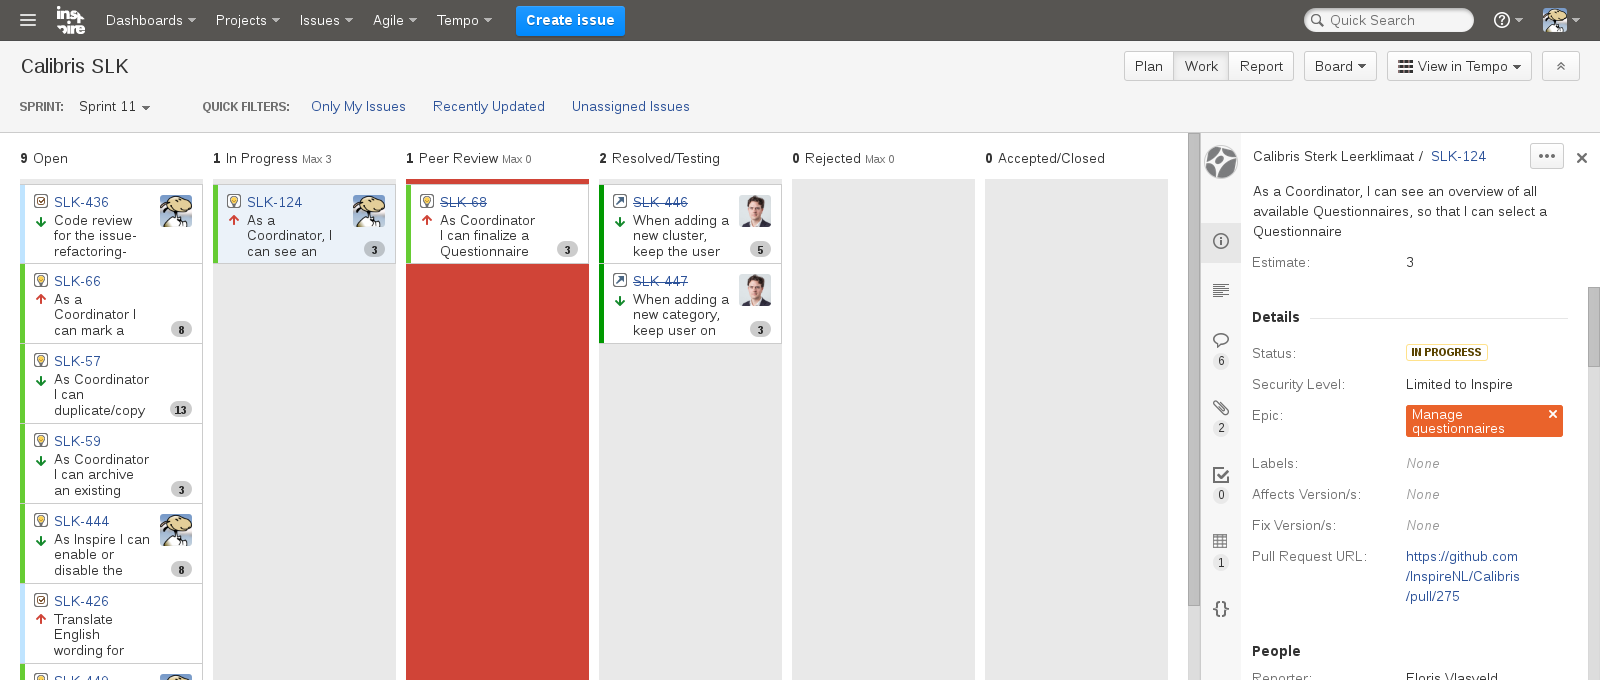
\includegraphics[scale=.30]{img/jira_agile_2.png}
 \caption{Vue du sprint en cours sur le module Agile de Jira}
 \label{fig.jira_agile2}
\end{figure}

Ce module, comme son nom l'indique, permet de gérer de façon efficace l'ensemble des tâches qui sont à effectuer sur les projets en cours. Il se décompose en trois vues :

\begin{description}
  \item[Plan] La vue Plan (voir \cref{fig.jira_agile1}) offre une vue globale de l'ensemble des tâches du sprint actuel mais également des sprints à venir. Les tâches peuvent également être éditées depuis cette interface afin, entre autre, de leurs affecter une difficulté (les nombres de la suite de Fibonacci sont ici utilisés), d'ajouter des commentaires, d'y joindre des documents/images ou d'y affecter une personne de l'équipe.
  \item[Work] Cette vue permet d'organiser les tâches du sprint en cours en suivant les différentes étapes de validation (voir \cref{fig.jira_agile2}). Chacune des tâches se trouve innitialement dans la colonne ``Open'', lors qu'un développeur sera assigné à une tâche (il peut également la choisir lui même) il la déplacera dans la seconde colonne ``In Progress'' et travaillera à sa résolution (en réutilisant la méthodologie précisée dans \cref{sec.git} via la création d'une nouvelle branche sur le dépôt). Lorsque la tâche est finalisée, celle-ci doit encore passer par l'étape ``Peer Review'' afin d'être vérifié par un tiers. Finalement elle sera soit acceptée (cinquième colonne) soit refusée (colonne six), soit renvoyée à l'étape ``Open'' si le second développeur estime que des développements complémentaires sont nécessaires pour la résolution de celle-ci.
  \item[Report] La troisième et dernière vue sert plus au manager. Celle-ci offre des graphiques et statistiques sur le déroulement des différents sprints, la vélocité de l'équipe ou encore la quantité de travail restant à effectuer.
\end{description}

Un système lié à la messagerie interne de l'entreprise (à savoir les comptes mails et de messagerie instantanée) permet à chacun de notifier un, plusieurs ou l'ensemble de ses collègues sur l'évolution ou une difficultée rencontrée sur l'une des tâches.

\subsubsection{Le module Tempo}

En remplacement de l'application Harvest\footnote{\url{http://www.getharvest.com/}} utilisée jusqu'alors, le module Tempo permet à chacun de suivre le temps passé sur chaque tâche. Fortement lié au module précédent, les développeurs et les manageurs peuvent ainsi constater si les estimations faites sur les tâches correspondent au temps utilisé pour leur résolution.

Ce module permet également de savoir quel travail sera facturé au client et de savoir sur quelles tâches le développeur a passé ses quarantes heures de travail hebdomadaires.

\subsection{En bref} 

D'une façon générale, l'ensemble de ces outils sert essentiellement à synchroniser et à garder informé l'ensemble des membres de l'équipe de l'état dans lequel se trouve un projet mais également du travail effectué par leurs collègues.

Quelques autres outils viennent également compléter certains aspects organisationnels tel que Google Calendar\footnote{\url{https://www.google.com/calendar/}} pour la planification des réunions et des évènements internes à l'entreprise ou la messagerie instantanée pour l'envoi rapide de notifications aux différents collaborateurs.

\chapter{Planning}

Afin de comprendre le déroulement du planning qui va suivre il me semble nécessaire de revenir sur la méthodologie employée au sein de Inspire pour la gestion des projets.

Les membres de l'équipe organisent leur travail en suivant scrupuleusement certaines spécificités des méthodologies Agile. Les cycles étant d'environ 2 semaine (suivant le type de projet et la charge de travail qu'il reste à faire sur ceux-ci).

Lors de la définition de mon sujet j'ai essentiellement souhaité travailler sur les technologies dites ``frontend'' (donc étant en grande partie coté navigateur) tel que Javascript, CSS ou encore DOM. Le projet Calibris m'a donc été confié car les tâches qui étaient à effectuer sur celui-ci étaient essentiellement tournées vers cet aspect.

Le travail que j'ai effectué sur peut aisément se subdiviser en plusieurs thème. Tout d'abord le projet Calibris, que je détaillerai en première partie. J'ai également rédigé un article concernant la technologie Websocket sur le blog officiel de Inspire.

\section{Calibris}

Le projet Calibris a occupé la majeure partie des six mois de travail effectués à Inspire. Initialement prévu comme un premier projet sur lequel me pencher au début de mon stage, j'ai finalement eu la possibilité de continuer à travailler dessus suite à l'ajout de nouveaux objectifs au fur et à mesure de l'accomplissement des tâches précédentes.

\begin{figure}[htp]
\centering

\includegraphics[scale=.60]{img/calibris.jpg}
 \caption{Calibris, l'un des clients de Inspire}
 \label{fig.jira_agile1}
\end{figure}

Je pourrais donc diviser l'ensemble du travail en trois grandes sections, le gestionnaire de création de questionnaires, la mise à jour vers Rails 4 et le portage d'une partie de l'interface sur mobile.

\subsection{Gestionnaire de questionnaires}

Cette première partie s'est déroulée sur trois sprints (soit environ huit semaines, mes sprints s'étallant sur un peu plus de deux semaines) dont une étape préalable. 

\begin{description}
  \item[Préparation] Étape de préparation comprenant entre autre : une revue générale des fonctionnalités et du fonctionnement global de l'application avec un collègue, une première compréhension du code et la lecture de nombreux tutoriels afin de me ré-imprégnier des méthodes et techniques du framework Ruby on Rails. Cette étape préalable s'est déroulée sur une semaine.
  \item[Sprint 1] Implémentation des premiers scénarios utilisateurs, scénarios qui avaient été définits avant mon stage (et qui attendaient donc une implémentation). Ce sprint a démarré suite à une réunion qui a permise de prioriser et de réorganiser ces scénarios. À l'issue de celui-ci un utilisateur pouvait créer, voir, détruire et modifier les questionnaires de l'applications ainsi que les trois niveaux les composants (catégories, clusters et questions). Ce sprint s'est déroulé sur environ deux semaines.
  \item[Sprint 2] Ce sprint était plus en laision avec les technologies que j'avais souhaité découvrir au sein de ce stage. L'idée était principalement de reprendre le travail effectué au sprint 1 et de rendre l'interface d'édition plus agréable à l'utilisation en minimisant les étapes nécessaire à l'édition de l'ensemble des éléments d'un questionnaire. De ce fait la création des éléments et sous-éléments ne passait plus par le chargement d'une nouvelle page mais par l'apparition d'un nouvel élément vide dès le clique sur le bouton ``création'', de même pour l'édition et la suppression des éléments. Le travail d'intégration étant assez conséquent ce sprint s'est étendu sur près de trois semaines.
  \item[Sprint 3] Ce dernier sprint concernait essentiellement les tâches d'intégration de l'ensemble des fonctionnalités précédemment mentionné dans le reste de l'interface. Cela passait essentiellement par la vérification des rôles ayant accès aux pages permettant l'édition des questionnaires, mais aussi la correction des nombreux tests et des formulaires permettant l'intégration des formulaires nouvellement créés au sein d'un projet (appelé ``enquête'' ou ``sondage'' dans l'application). Ce sprint comportait également un ensemble de scénarios utilisateurs qui ajoutaient des fonctionnalités de gestion sur les questionnaires même (tel que la duplication d'un questionnaire afin de servir de base à un autre ou l'archivage d'un questionnaire après son utilisation).
\end{description}

Cet ensemble de fonctionnalités étant liées au gestionnaire de questionnaire ont été finalisés au début du mois de mai.

\subsection{Passage à Rails 4}

Le projet Calibris est une application ayant été écrite sur la version trois du framework Ruby on Rails. La seconde tâche majeure que j'aurais à effectuer sur celui-ci consistera à migrer l'ensemble du code-source vers la version quatre. Cette volonté de migrer les projets vers les versions récentes du framework fait partie de la politique globale de l'agence Inspire afin d'éviter à avoir à maintenir un ensemble hétéroclite de versions (du framework mais aussi des modules, ou Gems).

Une autre raison est venue pousser au portage de Calibris sur RoR 4. La tâche suivant consiste à adapter une partie de l'application (en l'occurence toute l'interface servant à répondre aux questionnaires) afin de la rendre compatible pour une consultation des les appareils mobiles. La version quatre du framework intègre de nombreux outils facilitant grandement la tâche au développeur pour le portage d'un application sur ces appareils nomades (dont entre autre un astucieux algorytme permettant de détecter efficacement le type d'appareil et de rediriger l'utilisateur vers une vue adapté à son appareil).

Cette tâche s'est déroulée sur un seul et unique sprint (donc entre 2 et 3 semaines).

\subsection{Interface de réponse sur mobile}

Le projet Calibris possède deux grand rôles :
\begin{itemize}
  \item Il permet tout d'abord aux administrateurs de gérer des questionnaires, des entités (associations, entreprises), des utilisateurs et de sondages ou enquêtes via une unique interface web.
  \item Il permet également l'envois d'invitations (par email) aux utilisateurs afin que ceux-ci répondent aux questionnaire grâce à l'interface adaptée.  
\end{itemize}

Le but de cette tâche a donc été de porter la seconde partie de cette application sur les plateformes mobiles afin d'améliorer l'accessibilité aux utilisateurs souhaitant remplir le questionnaire rapidement sans avoir un accès direct à un ordinateur portable ou fixe.

J'ai décidé d'adapter cette partie de l'application en reprenant les feuilles de style existantes afin de rendre l'interface adaptative sur les différentes taille d'écran.

Plusieurs arguments sont venus appuyer cette décision :
\begin{itemize}
  \item L'interface actuelle n'est pas particulièrement complexe à adapter. Une grande partie des éléments étant déjà affichés sous forme de listes et l'interface générale étant organisé autour d'une unique colonne l'adaptation ne s'est pas concentrée sur la réorganisation du contenu.
  \item L'utilisation de feuilles de style adaptatives permet également d'éviter d'avoir à créer plusieurs vues pour les différents appareils et ainsi perdre du temps lors de la modification du contenu (qui devra alors se répercuter sur plusieurs fichiers en parallèle)
\end{itemize}

Initialement prévue sur deux semaines l'adaptation du code existant a finalement été plus facile que prévu et s'est déroulée en une seule semaine.

\subsection{Gestionnaire de questionnaires, ajouts}

Suite à l'ajout de l'ensemble de ces fonctionnalités, plusieurs modifications substantielles ont été apportées au gestionnaire de questionnaire. Celles-ci étants particulièrement destinées à l'amélioration de l'édition des questions lors de la création d'un formulaire.

\begin{figure}[htp]
\centering
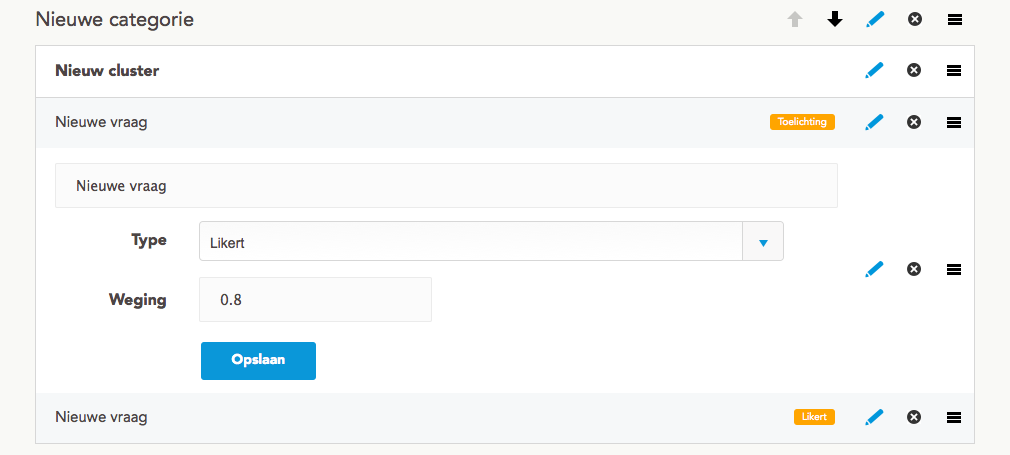
\includegraphics[scale=.45]{img/editor.png}
 \caption{Nouvelle interface d'édition des questions}
 \label{fig.editor}
\end{figure}

Un nouvel attribut a été ajouté au modèle \texttt{Question}, nommé \texttt{weight} il permet de donner une importance plus ou moins grande afin de pouvoir pondérer les réponses lors de l'analyse de celles-ci.

Afin d'ajouter ce nouvel élement un remaniement de l'interface était nécessaire. En effet le formulaire d'édition actuel ne laissait aucune place supplémentaire pour de nouvelles entrées.

Une étape préliminaire a donc été créée et consistait à adapter ce formulaire pour le rendre extensible. Le résultat, visible sur la \cref{fig.editor} permet de bien distinguer les différents items du formulaire (ici le champ pour la question en elle même, le type et le poids).

Suite à ça l'ajout du nouvel élément s'est fait suivant la méthodologie classique à tout projet Ruby on Rails.

\begin{enumerate}
  \item Ajout d'une Migration, pour annoncer un changement dans la base de donnée, ici une colonne \texttt{weight} contenant un nombre flottant (le poids étant compris entre 0.0 et 1.0) dans la table \texttt{questions}. Application de cette Migration pour mettre à jour la base de donnée.
  \item Ajout de validations dans le modèle pour prendre en compte les particularités de ce nouvel attribut. Voir \cref{fig.weight_validation}.
  
  \begin{figure}[h]
  \lstset{language=ruby}
  \begin{lstlisting}
validates :weight, numericality: { greater_than_or_equal_to: 0.0, less_than_or_equal_to: 1.0 }
  \end{lstlisting}
   \caption{Ajout de limites sur l'attribut \texttt{weight} du modèle Question}
  \label{fig.weight_validation}
  \end{figure}
  \item Ajout et/ou modification des contrôlleurs et vues existantes pour prendre en compte le nouvel attribut.

  \begin{figure}[h]
  \lstset{language=ruby}
  \begin{lstlisting}
.input
  = f.label :weight, t('questions.field.weight')
  = f.text_field :weight, "data-rule-required" => true
  \end{lstlisting}
   \caption{Nouvel élément dans le formulaire d'édition}
  \label{fig.weight_validation}
  \end{figure}
  
\end{enumerate}

\subsection{Correction et ajout des tests et ``Seeds''}

Suite à l'ajout de toutes ces fonctionnalités deux étapes sont nécessaires afin de les intégrer correctement au reste du projet.

Je devais tout d'abord m'assurer que toutes ces fonctionnalités étaient correctement testées. Pour plus d'informations sur cette partie voir la \cref{sec.tests}.

Les ``seeds'' de l'application ont dû être en partie réécrits pour prendre en compte les changements effectués dans la structure (et plus particulièrement dans les modèles).

  \begin{figure}[h]
  \lstset{language=ruby}
  \begin{lstlisting}
p "creating respondents"
25.times do |i|
  @finished_respondent = Respondent.create(
  email: "example@example.com",
  name: "Finished respondent #{i+1}",
  survey_id: @survey1.id
  )
end
  \end{lstlisting}
   \caption{Exemple de seed, génération de réponses aux questions des questionnaires}
  \label{fig.seeds}
  \end{figure}

Les fichiers ``seeds'' d'une application Ruby on Rails prennent la forme de scripts Ruby et sont sensés remplir les tables de la base de donnée lors du premier lancement de l'application (création des rôles par défaut, des projets de bases…). Ils sont également un excelent moyen supplémentaire de tester la viabilité de la structure de donnée dans un environnement controllé (en plus des tests).

Ces scripts sont placés dans le dossier \texttt{db/seeds/} et sont exécutés via la commande \\
\texttt{rake db:seed}.

Dans la \cref{fig.seeds} nous avons un extrait de l'un des ``seeds'' de Calibris permettant de créer 25 utilisateurs ayant répondu au questionnaire proposé. 

Répartit sur la totalité du stage ces deux étapes ont pris, en temps cumulé, environ deux à trois semaines de développement.

\subsection{Écriture de documentation}

Afin d'informer l'équipe de certaines modifications effectuées sur Calibris j'ai également complété la documentation interne au projet et la générale s'appliquant à l'ensemble des membres de Inspire.

J'ai pris soin d'expliquer mes changements sur la documentation de Calibris, ayant légèrement modifié les scripts de ``seeding'' et de création de base de donnée (afin de les adapters pour les différents clients du projet).

Le Wiki officiel de l'agence a également été complété par certains liens pouvant être utiles à tous concernant de bonne méthodes d'organisation et de programmation sur le framework Ruby on Rails.

Ruby on Rails réconseille toute écriture de documentation au sein du code source (à la manière de Doxygen) préférant le déclaration de méthodes et classes dites ``autodescriptives''. Le code source \cref{fig.autodesc} en est le témoin.

  \begin{figure}[h]
  \lstset{language=ruby}
  \begin{lstlisting}
def move_up
  @category.move_left unless @category.questionnaire.published?
  render nothing: true
end 
  \end{lstlisting}
   \caption{Méthode ayant un code ``autodescriptif''}
  \label{fig.autodesc}
  \end{figure}
  
Une personne n'ayant jamais fait de Ruby on Rails comprend ici assez facilement le sens de cette méthode.

\section{Rédaction d'un article sur la technologie Websocket}

Suite à la réalisation de l'ensemble des tâches m'ayant été assignés sur Calibris j'ai décidé de participer à la rédaction d'un article sur le blog de l'agence. La technologie Websocket me tenant particulièrement à cœur je l'ai alors proposé aux membres de l'agence afin d'avoir leurs approbation avant de commencer la rédaction.

N'ayant pas particulièrement de connaissances sur le domaine plusieurs jours de veilles et d'expérimentations ont été nécessaires avant de commencer la rédaction de l'article.

L'article est aujourd'hui disponible à cette adresse : \url{http://www.inspire.nl/blog/websockets-let-s-talk-about-real-time/}. Je ne détaillerai pas les spécificités techniques des Websockets, l'article étant déjà assez complet à ce sujet.

La veille, la rédaction, la correction et la publication de l'article m'a occupé un peu plus d'une semaine. Plusieurs jours supplémentaires ont été nécessaires pour expérimenter et mettre en place deux tutoriels (l'un en Javascript, l'autre en Rails) que j'ai intégré au sein de l'article. J'ai également ajouté 4 schémas à la publication finale pour en faciliter la lecture.

\chapter{Projets}

Au sein de ce chapitre je présenterai les différents projets sur lesquels j'ai pu travailler tout au long du stage, chacun d'entre eux sera composé de trois parties. Je commencerais par faire une présentation générale de l'application et de ses particularités. Puis je reviendrais sur les fonctionnalités qui sont soit à améliorer, soit à développer. J'apporterai par la suite quelques explications détaillées sur des particularités du développement. Finalement je ferais un retour personnel sur les apports de connaissances que j'ai pu avoir tout au long du projet.

\section{Calibris - Gestionnaire de questionnaire}

\label{sec:calibris}
Calibris est une application développée par Inspire servant à gestion et au remplissage de questionnaires auprès des membres d'une infrastructure.

Suite au développement de cette application un accord est trouvé entre Inspire et le client Innergo\footnote{\url{http://www.innergo.nl/}} afin de partager entre les deux entitées la propriété du code-source. Inspire est alors autorisée à continuer le développement sur l'application et de la revendre à d'autres entreprises.

\subsection{Contexte}

L'idée générale de l'application est de pouvoir importer des questionnaires, les affecter aux différentes structures organisationelles préalablement créées au sein de l'interface et de les transmettres aux collaborateurs de ces mêmes structures. 

Deux ensembles d'utilisateurs sont ici présents (voir \cref{fig.calibris_clients}) :
\begin{itemize}
  \item Ceux qui créent, publient et adminitrent les questionnaires, ce sont bien souvent les clients avec qui Inspire va travailler pour adapter l'application à leurs besoins. Pour le moment Inspire travaille avec Calibris\footnote{\url{http://www.calibris.nl/}} (le premier client, qui a également donné le nom à l'application), Innergo et ICSS.
  \item Ceux qui répondent aux questionnaires, bien souvent membres ou clients des organisations clientes de Inspire. 
\end{itemize}

\begin{figure}[h]
   \centering
\begin{tikzpicture}
\begin{scope}[xscale=2,yscale=1.5]
% description et nommage des noeuds 
\node (A) at (0,0) [circle, draw] {\Large{Calibris}};
\node (I) at (0,2) [rectangle,draw] {Inspire};
\node (C1) at (-3,1) [rectangle,draw] {Calibris};
\node (C2) at (-3,0) [rectangle,draw] {Innergo};
\node (C3) at (-3,-1) [rectangle,draw] {ICSS};
\node (T) at (-3,2) {\textbf{Clients/Administrateurs}};
\node (T) at (3,2) {\textbf{Utilisateurs passifs}};
\node (R) at (3,0) [rectangle,draw] {Respondents};
\draw[dashed, ->]  (I) -- (A);
\draw (C1) -- (A);
\draw (C2) -- (A);
\draw (C3) -- (A);
\draw[->] (R) -- (A);
\end{scope}
\end{tikzpicture}
\caption{Vue générale des utilisateurs actuels de l'application Calibris} 
\label{fig.calibris_clients}
\end{figure}

L'interface de l'application permet de gérer les structures ainsi que les membres les composants, des rôles pouvant êtres appliqués à certains d'entre eux afin de déléguer certains pouvoirs. 

Nous retrouvons ici trois rôles clefs dans l'administration de Calibris :
\begin{description}
  \item[Administrateurs] Ils ont un accès complet à l'interface et peuvent à tout moment créer/modifier/supprimer les questionnaires et utilisateurs. Ils peuvent créer une nouvelle organisation au sein de l'application. 
  \item[Organisation Managers] Peuvent administrer les organisations et créer des nouveaux projets en leurs sein.
  \item[Titulaires de permis] Ont l'autorisation d'administrer un projet au sein d'une organisation.
\end{description}
  
Les utilisateurs répondants aux questionnaires le font de façon anonyme via la réception d'un lien comportant un numéro unique de session au sein d'un email.

\subsection{Structure d'un questionnaire}

Les questionnaires sont construit suivant trois niveaux. 

\begin{enumerate}
  \item Les catégories qui font office de séparateur permettant de regrouper les questions par thèmes.
  \item Les ``clusters'', sous-catégories, ils permettent d'associer des ensembles de questions traitant des sujets similaires.
  \item Les questions, étants pour le moment de deux types, à réponse ouverte (l'utilisateur a le choix de compléter textuellement sa réponse) ou par une appréciation à cinq niveaux allant de -2 à 2.
\end{enumerate}

Chaque questionnaire possède un titre et une durée moyenne de remplissage arbitrairement définie par le créateur. Les catégories et ``clusters'' possèdent tous deux un nom et sont stockés suivant la même structure dans la base de donnée (un ``cluster'' étant une catégorie ayant comme parent une catégorie).

Les questions possèdent un type, une étiquette (contenant la question en elle même), un poids (permettant de pondérer leurs réponses) et un ``cluster'' parent.

Les questionnaires sont intégrés dans l'application via l'importation de tableaux au format CSV (format de tableau simplifié où les cases sont séparées par des virgules) ou Excel.

\begin{figure}[htp]
\centering
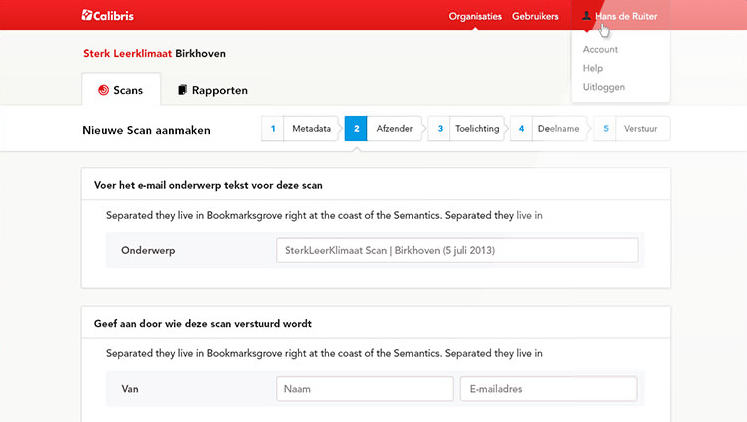
\includegraphics[scale=0.6]{img/calibris1.png}
 \caption{Création d'un nouveau projet de questionnaire sur Calibris}
 \label{fig.calibris1}
\end{figure}

\begin{figure}[htp]
\centering
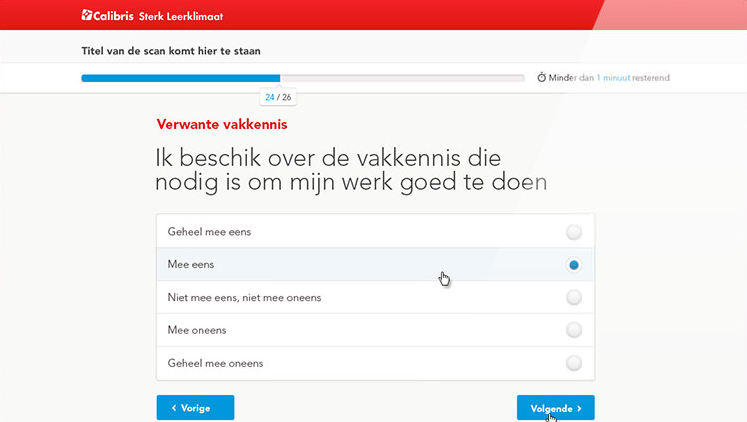
\includegraphics[scale=0.6]{img/calibris2.png}
 \caption{Interface de réponse au questionnaire sur Calibris}
 \label{fig.calibris2}
\end{figure}

\subsection{Travail à effectuer}

Le travail qui m'était demandé devait s'effectuer en deux temps. Inspire ayant acquit une partie des droits d'exploitation de l'application celle-ci souhaite ajouter de nouvelles fonctionnalités qu'elle pourra vendre à de nouveaux clients.

Je devait tout d'abord développer une interface complète permettant de créer, administrer et modifier des questionnaires sans avoir à les importer depuis un fichier externe. Le but général étant donc d'intégrer une interface dynamique permetant la création des différents niveaux (catégories, ``clusters'' et questions) et leurs réorganisations en vue d'une futur publication.

La seconde étape consistant à intégrer cette nouvelle fonctionnalité au reste de l'application via l'interfacage avec les formulaires de gestion des réponses et des droits des utilisateurs.

Pour la réalisation de ce projet je suis épaulée par deux développeurs ayant déjà travaillés plusieurs fois sur le code existant. Ceux-ci m'ont également expliqué en détail de fonctionnement de l'applicaion et des tâches qui m'étaient confiées.

\subsection{Développement}

Dans cette section je reviendrai globalement sur le travail que j'ai eu à effectuer jusqu'alors sur Calibris. Par la suite je détaillerai quelques points technique que j'estime intéressant de préciser.

\subsubsection{Développement général}

Le développement de l'interface d'édition des questionnaire n'a pas réellement causée de grand changement dans la structure même du modèle de données de l'application. L'idée ici étant de pouvoir modifier le contenue des données. Cependant une refactorisation du code source a été nécessaire pour résoudre un problème de structure entre les différents niveaux de l'application.

J'ai donc commencé le développement de façon incrémental via l'implémentation des différentes actions possibles sur chaques types d'éléments du questionnaire. L'idée générale étant de supporter l'ensemble des actions CRUD (create, read, update, delete) pour chacun d'entre eux.

Au fur et à mesure de l'implémentation de ces fonctionnalités j'ai fait valider mon travail par des collègues qui connaissaient déjà particulièrement bien le code existant.

\subsubsection{Utilisation des imbrications d'ensembles}
\label{sec.aws}

Comme vu dans le chapitre précédent, un questionnaire possède trois niveaux dont les éléments possèdent chacun un ordre d'apparition bien précis. La structure d'un questionnaire peut donc se représenter par un arbre.

Suite à l'implémentation des première fonctionnalités il est apparu que la structure offerte par défaut pour la liaison des différents modèles de données au sein de Ruby on Rails ne permettait pas d'assurer cet notion d'ordre. De plus la réorganisation de l'ordre des éléments serait source d'une importante activité au niveau de la base de donnée afin de correctement mettre à jour les positions de tout les éléments.

Afin de remédier à ce problème l'équipe a décidée d'utiliser un \textit{gem} exploitant la structure des imbrications d'ensembles\footnote{En informatique, l'imbrication d'ensembles, nested sets en anglais, est une technique pour représenter des données hiérarchisées dans une base de données relationnelle. En substance, elle consiste à attribuer à chaque nœud deux bornes, dite gauche et droite, qui permettent de statuer sur les liens de parentés entre les différents nœuds. Source \url{http://fr.wikipedia.org/wiki/Imbrication_d'ensembles}}

\begin{figure}[htp]
\centering
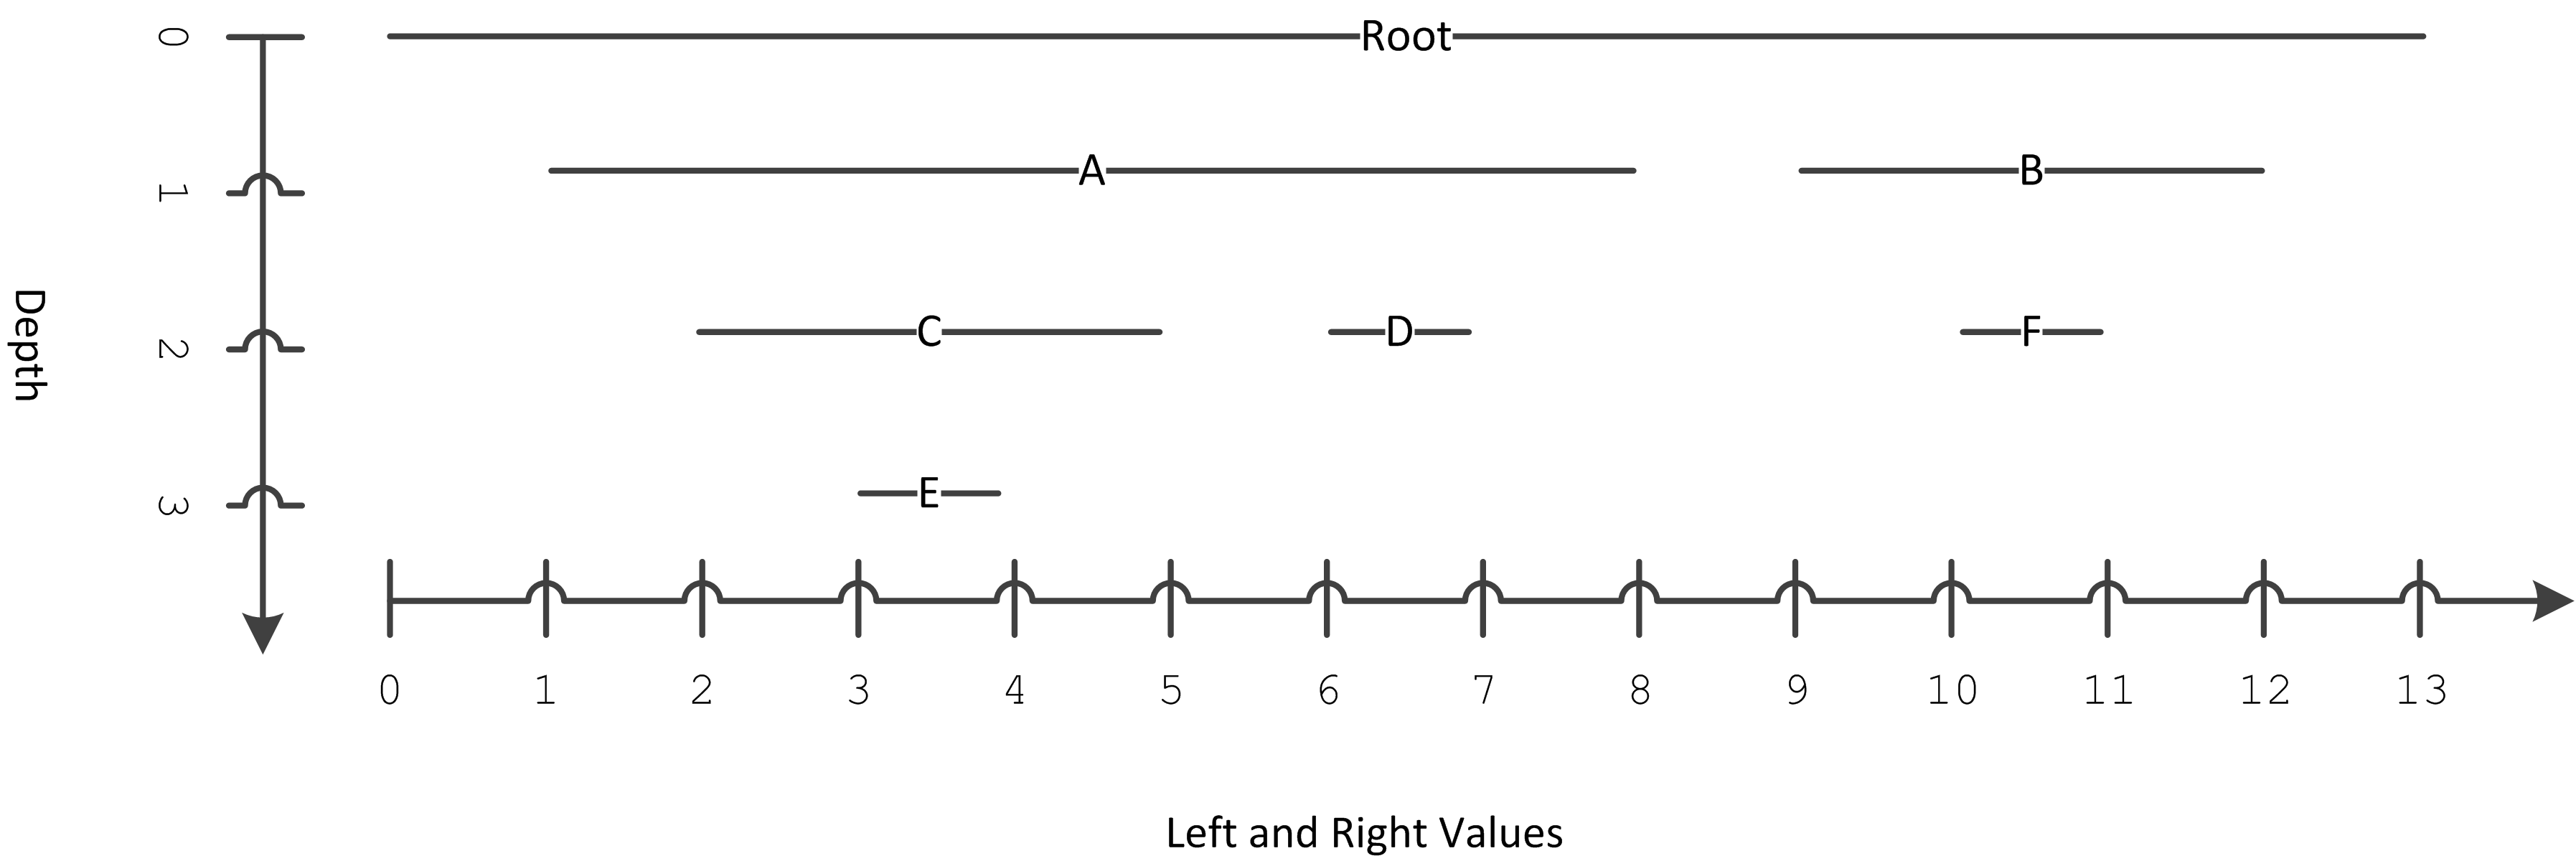
\includegraphics[scale=.12]{img/nested1.png}
\caption{Représentation schématique des nœuds d'un arbre sous forme d'imbrication d'ensembles}
\label{img:nested1}
\end{figure}

L'idée générale peut être schématisée par la \cref{img:nested1}. Chaque nœud de l'arbre possède une valeur ``gauche'' et ``droite'' qui sont respectivement plus grande et plus petite que les valeurs de son propre parent. Ici des nombres entiers sont utilisés afin de faciliter la lecture et l'écriture des valeurs dans une base de donnée SQL mais il est préférable d'utiliser des nombres réels afin d'éviter de mettre à jour de nombreuses valeurs lors du déplacement, de l'ajout ou de la suppresion de nœuds.

Cette structure de données permet également de connaitre de façon très rapide tout les éléments enfants d'un certain nœud via une simple requète d'ordre. Par exemple pour connaitre les enfants de A (soit C, D et E) il suffit de faire une requète similaire à la \cref{fig.nestedsql}.

\begin{figure}[h]
\lstset{language=sql}
\begin{lstlisting}
select * from nodes where lft > 1 and rgt < 8
\end{lstlisting}
 \caption{Exemple de requète SQL sur un arbre ordonné par les ensembles imbriqués}
 \label{fig.nestedsql}
\end{figure}

L'ensemble de ces fonctionnalités sont gérées de façon transparentes par le \textit{gem} AwesomeNestedSet\footnote{\url{https://github.com/collectiveidea/awesome_nested_set}}. Celui-ci permet de convertir un, ou des, modèle(s) d'un projet Ruby on Rails en nœud utilisant cette structure.

\begin{figure}[h]
\lstset{language=ruby}
\begin{lstlisting}
def create
  set_parent_category
  @category = @questionnaire.categories.build(name: name))

  if @category.save
    @category.move_to_child_of(@parent_category) if @parent_category
    flash[:notice] = t('categories.create.success')
  else
    flash[:alert] = t('categories.create.failure')
  end

  redirect_to @questionnaire
end
\end{lstlisting}
 \caption{Exemple de méthode utilisant AwesomeNestedSet}
 \label{fig.nestedrail}
\end{figure}

La \cref{fig.nestedrail} présente une action d'un contrôleur de l'application Calibris exploitant la fonctionnalités \texttt{move\_to\_child\_of} offerte par la bibliothèque. Ici l'ensemble des modifications faites à la base de donnée est cachée et sont gérées intelligement par le \textit{gem}.

\subsubsection{Utilisation des \texttt{remote}}

Un autre élément intéressant inhérant à Ruby on Rails et exploité à de multiples reprises dans l'application est la balise \texttt{remote}.

Afin de bien comprendre l'utilité de cette fonctionnalité il faut tout d'abord détailler un peu le fonctionnement du Modèle-Vue-Controlleur au sein de Ruby on Rails.

\paragraph{Le chargement d'une page} passe systématiquement par l'utilisation d'une route unique et prédéfinie dans la configuration de l'application. Nous allons ici prendre l'exemple du chargement de la page \textit{index} du contrôleur \textit{QuestionnaireController}.

Cette page possède comme rôle de lister l'ensemble des questionnaires actuellement présents dans la base de donnée de l'application. Elle est accessible par le chemin \texttt{questionnaires\_path}, chemin qui retourne une URL correspondant à l'adresse exacte de la page (dans notre cas il s'agit de \url{http://localhost:3000/questionnaires}).

Lorsque nous allons visiter cette URL (via un lien interne à l'application ou en rentrant directement l'adresse dans la barre du navigateur), le framework va alors tenter de charger plusieurs éléments.

\begin{enumerate}
  \item Il va tout d'abord interroger le Controlleur correspondant à l'URL interrogée, dans notre cas il s'agit de QuestionnaireController.
  \item Puis il va cherche l'action spécifique à exécuter au sein du Controlleur. Si aucune action n'est spécifiée (ce qui est ici le cas puisque rien n'a été précisé à la fin de l'URL) c'est l'action \texttt{index} qui est exécutée.
  \item Le framework va alors exécuter la méthode \texttt{index} du contrôleur, celle-ci s'occupera du rendu de la page \texttt{index.html}, laquelle sera renvoyée au navigateur.
\end{enumerate}

\paragraph{Dans certains cas} nous ne souhaitons pas générer une page XHTML classique mais plutôt exécuter du code Javascript afin d'effectuer une transformation particulière sur la page courante. Dans ce cas précis nous ne voulons pas appeler l'action (qui, rappelons le, correspond à une méthode du Controlleur) via le chargement d'une page mais plutôt de façon asynchrone via une requète Ajax\footnote{L'architecture informatique Ajax (acronyme d'Asynchronous JavaScript and XML) permet de construire des applications Web et des sites web dynamiques interactifs sur le poste client en se servant de différentes technologies ajoutées aux navigateurs web entre 1995 et 2005. \url{http://fr.wikipedia.org/wiki/Asynchronous_JavaScript_and_XML}}. 

\paragraph{L'ajout d'un lien} dans une vue Rails se fait d'une façon similaire au code de la \cref{fig.link}. Ici nous appelons la fonction \texttt{link\_to} qui génèrera une balise \texttt{a} possédant un titre et une classe. La valeur du lien (correspondant au contenu de l'attribut \texttt{href}) est le résultat de la fonction \texttt{questionnaires\_path}.

Ce code génèrera un lien XHTML similaire à la \cref{fig.link2}.

\begin{figure}[h]
\lstset{language=ruby}
\begin{lstlisting}
link_to questionnaires_path, 
  title: t('questionnaires.title'), 
  class: 'questionnaire-edit'
\end{lstlisting}
 \caption{Extrait d'une vue s'occupant de la génération d'un lien}
 \label{fig.link}
\end{figure}

\begin{figure}[h]
\lstset{language=xml}
\begin{lstlisting}
<a href="http://localhost:3000/questionnaires/" 
   title="Les Questionnaires" 
   class="questionnaire-edit"/>
\end{lstlisting}
 \caption{Exemple de code généré à partir de la \cref{fig.link}}
 \label{fig.link2}
\end{figure}

\paragraph{L'ajout du paramètre \texttt{remote}} à la fonction \texttt{link\_to} va permettre de changer radicalement le comportement du lien. En effet, lors du clic sur celui-ci, le navigateur ne va pas se diriger vers la nouvelle page mais plutôt générer une requête Ajax qui ira interroger l'action en question dans la classe QuestionControlleur. Le résultat attendu n'est donc pas une page XHTML mais plutôt du code Javascript pouvant être traité par le navigateur lors de la génération de la réponse par le serveur.

L'ensemble de ce mécanisme est automatiquement généré par le framework Ruby on Rails dès le simple ajout de cet attribut.

Lors de mon développement j'ai donc utilisé à mainte reprises ce mécanisme afin de pouvoir remplacer des éléments du contenu des questionnaires par un formulaire d'édition. De cette façon l'utilisateur n'a qu'à cliquer directement sur l'élément pour que celui-ci soit remplacé par une balise d'édition permettant la modification dynamique de la valeur du champ sans rechargement de page.  

\subsubsection{Utilisation de jQuery Sortable}

La bibliothèque jQuery Sortable\footnote{\url{http://jqueryui.com/sortable/}} est une extension à la bibliothèque jQuery permettant la réorganisation des éléments d'une page XHTML via le déplacement sous forme de ``drag \& drop'' des blocs en question.

Après avoir correctement chargé les deux librairies (jQuery et jQuery Sortable) un petit peu de Javascript est à rédiger afin de faire le lien avec les éléments que nous souhaitons animer.

Le but ici étant de pouvoir réorganiser les différents éléments du questionnaire en cours d'édition (les catégories, clusters et questions) puis de sauvegarder ces mêmes modifications sur le serveur.

La déclaration d'une liste en tant qu'éléments ``sortables'' est assez simple et le comportement peut être facilement personnalisé. Comme la \cref{fig.sort1} le montre l'idée est simplement de rechercher un élément appelé ``parent'' qui servira de conteneur aux déplacement des blocs. Nous déclarons ensuite l'ensemble des enfants qui pourront être déplacés via l'utilisation d'un second sélecteur (ici définit par la clef \texttt{items}).

La clef \texttt{update} permet d'appeler une fonction Javascript particulière lorsque le déplacement est terminé (pour, par exemple, permettre de sauvegarder les modifications sur le serveur). Finalement, le mot clef \texttt{handle} permet de définir une zone sur chaque élément déplacable qui servira de poignée pour faciliter leurs réorganisation.

\begin{figure}[h]
%\lstset{language=js}
\begin{lstlisting}
$(".container.total_scores.questionnaires.sortable").sortable
    items: ".category_sortable"
    update: sortCategory
    handle: "th.score.grip"
\end{lstlisting}
 \caption{Déclaration d'une liste d'éléments ``sortables''}
 \label{fig.sort1}
\end{figure}

Dans mon cas il fallait que j'envois la nouvelle position de l'élément changé afin de mettre à jour l'arbre déclaré dans la base de donnée. Pour cela, chaque élément affiché possède un identifiant unique qui se trouve être celui issue de la base de donnée. Ainsi lors de la mise à jour je n'avait qu'à récupérer l'identifiant de l'élément parent, de l'élément à gauche et, si possible de l'élément à droite (dans le cas particulier ou l'élément serait déplacé en tout début de ``sous-liste'') puis de mettre à jour correctement mon modèle de donnée à partir de ces informations.

Le parent est ici également envoyé car nous avons autorisé le déplacement d'un élément d'un sous-branche à une autre.

\begin{figure}[h]
%\lstset{language=js}
\begin{lstlisting}
sortQuestion = (event, ui) ->
  items = $(this)
  params = {}
  if ui.item.context.className is "question_sortable"
    context = ui.item.context
    params["parent"] = context.parentNode.parentNode.parentNode.parentNode.id
    if context.previousElementSibling and context.previousElementSibling.id isnt ""
      params["previous"] = context.previousElementSibling.id
    if context.nextElementSibling and context.nextElementSibling.id isnt ""
      params["next"] = context.nextElementSibling.id 
  $.ajax
    url: ui.item.data("sort-url")
    type: "post"
    data: params
    dataType: "script"
    complete: (request) ->
      items.effect "highlight"
      return
\end{lstlisting}
 \caption{Mise à jour des informations lors du déplacement d'une question}
 \label{fig.sort2}
\end{figure}

Dans l'exemple de la \cref{fig.sort2} nous pouvons observer deux étapes. Tout d'abord la fonction va tenter de récupérer toutes les informations nécessaires à la bonne compréhension de la nouvelle proposition de l'élément en récupérant les identifiants des éléments à gauche et à droite (respectivement récupérés grâce à l'utilisation de la primitive DOM\footnote{Le Document Object Model (ou DOM) est un standard du W3C qui décrit une interface indépendante de tout langage de programmation et de toute plate-forme, permettant à des programmes informatiques et à des scripts d'accéder ou de mettre à jour le contenu, la structure ou le style de documents XML et HTML1. Le document peut ensuite être traité et les résultats de ces traitements peuvent être réincorporés dans le document tel qu'il sera présenté. Source \url{http://fr.wikipedia.org/wiki/Document_Object_Model}} \texttt{previousElementSibiling} et \texttt{nextElementSibling} et le parent.

Par la suite nous envoyons une simple requête Ajax vers le serveur avec ces informations et nous affichons un petit effet de surlignage (``highlight'') afin de confirmer la bonne prise en compte des informations.

La méthode \texttt{sort} Ruby on Rails présentée \cref{fig.sort3} permet de comprendre facilement comment les informations fraichement récupérées du navigateur vont servir à mettre à jour la base de donnée. 

Ici nous réutilisons des primitives du \textit{gem} AwesomeNestedSet présenté en \cref{sec.aws}. Tout d'abord nous affectons notre élément déplacé (ici une question) à son nouveau parent avant de le déplacer à gauche, ou a droite d'un de ses éléments frères suivant sa position dans la sous branche.

Cet méthode peut ici être facilement testée en vérifiant les positions de chaques élément après un déplacement dont le résultat est connu.

\begin{figure}[h]
\lstset{language=ruby}
\begin{lstlisting}
def sort
  @category = Category.find(params[:parent])

  @question.category = @category
  @question.save

  if params[:previous]
      @question.move_to_right_of params[:previous].to_i
  elsif params[:next]
      @question.move_to_left_of params[:next].to_i
  end

  render nothing: true
end
\end{lstlisting}
 \caption{Mise à jour des informations lors du déplacement d'une question}
 \label{fig.sort3}
\end{figure}

\section{Calibris - Passage à Rails 4} 

\subsection{Travail à effectuer}

La migration d'une application en Rails 4 peut se décomposer en plusieurs étapes. 

L'utilisation des tests pour couvrir notre code permet dans notre cas de détecter toute régression introduite par la mise à jour ce qui a été très utile pendant le portage du code.

La mise à jour d'un projet vers une nouvelle version se déroule généralement en trois temps :
\begin{itemize}
  \item Tout d'abord mettre à jour le numéro de version des libraries et Gem utilisées par le projet puis utiliser \texttt{bundle} pour appliquer ces modifications.
  \item Corriger une à une toutes les erreurs rencontrées afin de stabiliser et porter progressivement l'application sur la nouvelle base applicative.
  \item Exécuter la suite de tests afin de détecter toutes les régressions introduites et les corriger une à une.
\end{itemize}

Afin de ne pas déranger le reste de l'équipe cette migration sera faite dans une branche indépendante qui sera ``mergée'' avec la branche principale lorsque le travail sera accomplis.

\subsection{Développement}

\subsection{Mise à jour du Gemfile}

La première étape consiste donc à migrer l'application sur un nouveau socle comprenant des versions plus à jour des bibliothèques utilisées.

Comme précisé dans les notions préalables tout projet Rails comprend un fichier Gemfile qui définit l'ensemble des dépendances utilisées dans le projet. Ici il s'agit :
\begin{itemize}
  \item Soit de trouver une version compatible avec la version de Rails utilisée et de l'écrire en dur dans le fichier.
  
    \begin{figure}[h]
    \lstset{language=ruby}
    \begin{lstlisting}
gem 'awesome_nested_set', '~> 3.0.0.rc.5'
    \end{lstlisting}
     \caption{Gem chargé avec un numéro de version fixe}
    \end{figure}
    
  \item Soit de ne pas spécifier de version et de laisser le résolveur de dépendances le faire lui même.
  
    \begin{figure}[h]
    \lstset{language=ruby}
    \begin{lstlisting}
gem 'devise'
    \end{lstlisting}
     \caption{Gem dont le numéro de version est déclaré dynamiquement}
    \end{figure}
\end{itemize}

Pour le projet Calibris il faut le faire au cas par cas, certains Gem (tel que \texttt{awesome-nested-set}) ne possèdent pas encore de version par défaut étant pleinement compatible avec Rails 4, il faut donc forcer une version en développement.

\subsection{Correction des erreurs}

Il faut par la suite suivre les remarques et conseils donnés sur les Wiki et documentations des Gem mis à jour. Ils sont bien souvent une d'une précieuse aide pour résoudre les problèmes créés à la migration. 

Dans notre cas nous avons spécialement recontré des erreurs de syntaxes amenées avec l'utilisation de la nouvelle version de Ruby.

\subsubsection{Strong Parameters}

Rails 4 amène l'utilisation native des ``Strong Parameters'' dans l'implémentation de ses contrôleurs. Cet outil applique un filtre sur les paramètres reçus depuis le navigateur pour ne laisser passer que ceux pouvant intéresser le contrôleur en question.

Celà s'implémente assez facilement, l'idée étant de ne plus accepter directement dans les actions du contrôleur les tableaux de paramètres renvoyés par le navigateur mais de les passer auparavant dans une méthode intermédiaire faisant office de filtre.

Le principe a énormément été simplifié dans la dernière version. À chaque fois que nous manipulons les attributs d'un de nos modèles dans le contrôleur nous ne passons non pas en paramètre le tableau d'attributs mais une méthode privée qui va retourner un tableau ``filtré'' ne contenant que les attributs dont la modification est autorisée.

    \begin{figure}[h]
    \lstset{language=ruby}
    \begin{lstlisting}
// Here we update the attributes of a question
def update
  unless @question.update_attributes(question_params)
    set_question
  end
end

private

// And here we filter the attributes 
def question_params
  params.require(:question).permit(:label, :kind)
end
    \end{lstlisting}
     \caption{Utilisation des Strong Parameters au sein du contrôleur Question}
    \end{figure}
    
Calibris utilisais déjà un Gem intégrant cette fonctionnalité dans les versions précédentes de Rails. La migration n'a donc pas été très difficile, le code source des contrôleurs ayant déjà été formaté correctement avant la mise à jour.
    
\subsubsection{Reste du code}

Le reste des mises à jour concernait en grande partie des erreurs de syntaxe et des dépréciations de code.

Par exemple l'attribut \texttt{:order} (permettant de préciser dans quel ordre seront retournés certaines colonnes lorsque Rails interrogera la base de donnée depuis ce modèle) a été retiré lors de la définition des attributs des modèles. Celui-ci est remplacé par un ``bloc de code'' \footnote{Un ensemble d'instructions entourées par des accolades ou les mots clefs \texttt{do} et \texttt{end}} Ruby le tout entouré dans une ``lambda''.

    \begin{figure}[h]
    \lstset{language=ruby}
    \begin{lstlisting}
// Ancienne syntaxe
has_many :questions, order: 'questions.lft'
// Nouvelle syntaxe
has_many :questions, -> { order('questions.lft') }
    \end{lstlisting}
     \caption{Nouvelle syntaxe pour l'insertion de blocs de code dans les attributs d'un modèle}
    \end{figure}
    
Finalement, le code étant assez récent les autres corrections n'ont été que mineures.

\subsection{Exécution des tests}

L'exécution des tests (Cucumber et R-Spec) ont permis de détecter des régressions apparues suite à la mise à jour des Gem et du framework Rails.

C'est ici que nous pouvons pleinement apprécier les avantages apportés par la couverture de code grâce aux tests. En travaillant avec cette sécurité nous pouvons être sur de ne perdre aucune fonctionnalité lors de migrations importantes tel que la mise à jour vers une nouvelle version majeure du framework sous-jacent.

\subsection*{Conclusion}

La mise à jour d'une application Rails est toujours une étape délicate. La stabilisation du code source nous a ici pris un peu plus d'une semaine. Après vérification, la branche \texttt{master\_update} a été fusionnée avec la branche \texttt{master} quelques jours après et l'ensemble du projet tourne désormais sur cette nouvelle version.

\section{Calibris - Adaptation pour la version mobile}

\subsection{Travail à effectuer}

La dernière étape consitait à adapter une partie de l'interface afin de la rendre disponible pour les mobiles. Ici il a avant tout fallu décider par quel moyen l'adaptation allait se faire.

Lors du portage d'une application Web sur mobile, plusieurs méthodes peuvent être utilisées :
\begin{enumerate}
  \item Nous pouvons tout d'abord utiliser des outils tel que PhoneGap qui permettrent de générer et de packager des applications pour les différentes plateformes (iOS, Android, Windows Phone…) ici nous quittons donc le traditionnel navigateur Web pour passer sur la simulation d'une application native.
  \item Sur le framework Rails (comme sur de nombreux autres frameworks Web) il y a également possibilité de générer une interface adaptée au type de client (par la détection du type de navigateur et de plateforme). Celà passe par l'écriture de vues distinctes comportant chacunes des contenus différents (le plus souvent moins d'informations sont à afficher pour un rendu sur un écran de plus petite taille).
  \item Finalement il y a possibilité de rendre l'interface totallement adaptative en changeant dynamiquement la taille des éléments au fur suivant la taille de l'écran. Cette méthode appelée ``responsive design'' permet de n'avoir qu'un seul contenu et de ne travailler que sur la mise en forme de celui-ci.
\end{enumerate}

Dans mon cas j'ai préféré prendre la dernière solution pour les raisons que j'ai précisé dans le planning (le style de l'interface existante pouvant être facilement transformé en ``responsive'').

\begin{figure}[htp]
\centering
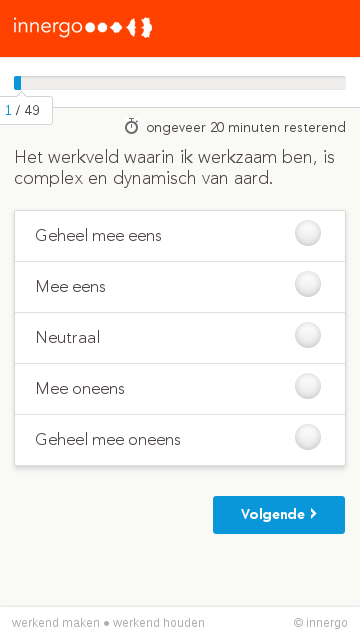
\includegraphics[scale=0.5]{img/calibris3.png}
 \caption{L'interface de réponse aux questionnaire sur mobile}
 \label{fig.calibris3}
\end{figure}

\subsection{Développement}

Dans cette partie je détaillerai certaines manipulations que j'ai eu l'occasion de faire lors de l'adaptation de l'interface pour le passage sur les appareils mobiles.

Ici je n'ai pas particulièrement utilisé d'outils du framework Ruby on Rails pour parvenir à mes fins. Au contraire j'ai préféré me reposer sur les technologies proposées par HTML5 tel que les les ``media-queries CSS3''\footnote{\url{http://www.w3.org/TR/css3-mediaqueries/}} ou certaines définitions CSS.

\subsubsection{media-queries CSS3}

Les technologies ``media-queries'' permettent d'adapter les propriétés CSS qui seront appliquées aux éléments de la page en fonction de variables d'environnement détectées tel que la résolution de rendu de la page, l'orientation de l'écran ou encore le support de certaines games de couleurs.

Elle peuvent être définies sur deux niveaux :
\begin{itemize}
  \item Soit dans le HTML même avec le chargement d'une feuille CSS spécifique aux variables précédement énoncées.
  \begin{figure}[h]
  \lstset{language=html}
  \begin{lstlisting}
<link 
  rel="stylesheet" 
  media="screen and (max-width: 640px)" 
  href="smallscreen.css" 
  type="text/css" />
  \end{lstlisting}
   \caption{Le chargement d'une feuille CSS spécifique au sein du code HTML}
   \label{fig.sort3}
  \end{figure}
  
    Ici le navigateur va donc charger la feuille de style \texttt{smallscreen.css} si la résolution de l'écran est inférieur à 640px en largeur.
  \item Mais nous pouvons également définir cette définition au sein de notre feuille de style.
  
  \begin{figure}[h]
  \lstset{language=html}
  \begin{lstlisting}
.bloc {
  background-color: red;
}
  
@media screen and (max-width: 640px) {
  .bloc {
    background-color: blue;
  }
}
  \end{lstlisting}
   \caption{L'application d'une media-query au sein d'une feuille de style}
   \label{fig.sort3}
  \end{figure}
  
  Une fois notre media-query définie il ne nous reste plus qu'à appliquer des nouveaux attributs qui viendront remplacer les valeurs des anciens attributs (le C de CSS voulant dire ``cascade'').
  
  L'exemple précédent permet de changer la couleur d'un simple élément lorsque qu'il est affiché sur un petit écran (passant ici de rouge à bleu).

\end{itemize}

Une fois les media-queries mises en places il ne nous reste plus qu'à définir le comportement de nos éléments sur notre page affichée sur mobile.

Quelques rêgles sont généralement suivies afin d'adapter efficacement les pages web :
\begin{itemize}
  \item La taille des polices est légèrement augmentée afin d'en faciliter la lecture.
  \item D'une façon plus générale c'est toute l'interface qui va être grossie, en grande partie pour faciliter la navigation (taille des boutons des menus). Le sélecteur devenant bien souvent le doigt de l'usager et non plus le curseur de la souris.
  \item Certaine réorganisations de contenu sont également à prévoir afin de faciliter l'exploration des divers éléments du site web (remplacement de listes simples par des listes déroulantes, séparation de textes longs en onglets).
\end{itemize}

Pour le cas de Calibris ce sont essentiellement les deux premiers facteurs qui ont été mis en place. Ainsi la taille du texte des titres et des questions affichés ont été adaptés.

\subsubsection{Adaptation des éléments}

Un élément intéressant à mentionner concerne la taille et la résolution des images. Ces deux facteurs ayant un impact important lors du rendu sur des terminaux différents.

Avec l'arrivée des écrans dits ``à haute définition'' sur les mobiles nous chamboulons totalement les densités d'affichage des textes et images au sein des pages web. L'unité CSS ``pixel'' ne se calquant plus du tout sur l'affiche réel d'un pixel à l'écran. Il est donc préférable d'utiliser des unités plus réalistes tel que le \texttt{em} qui est définit à partir de la taille des caractères de l'élément courant.

La \cref{fig.resolution} illustre parfaitement les soucis que nous pouvons avoir avec le rendu des images sur les écrans haute résolution. 

\begin{itemize}
  \item La première illustre l'affichage d'un icone de 8 par 8 pixels sur un écran basse résolution. Il est ici parfaitement affiché, les pixels de l'image d'alignant parfaitement sur ceux de l'écran.
  \item Sur la seconde image nus tentons d'afficher le même icone sur un écran haute résolution, nous voyons que les pixels agrandis de l'image d'origine chevauchent ceux de l'écran. Le navigateur va alors tenter d'interpoler ceux-ci créant un effet de flou lors du rendu.
  \item Sur la dernière image, nous chargeons la version vectorielle de l'icone, le navigateur va alors générer une image ayant la résolution native de l'écran.
\end{itemize}

\begin{figure}[htp]
\centering

\includegraphics[scale=0.9]{img/reso1.png}
 \caption{Rendu d'une forme selon les trois principes énoncés}
 \label{fig.resolution}
\end{figure}

Pour les images, nous rencontrons le même soucis. Contrairement aux textes, les images ont toujours tendances à s'afficher en suivant la résolution réelle de l'écran (un pixel de l'image équivalent à un pixel réel). Pourtant il arrive bien souvent aux développeurs de fixer leurs tailles afin de s'assurer de leurs bon placement dans la page. Lors du passage sur mobile, la résolution étant beaucoup plus dense, leurs rendu s'en trouve chamboulé (une icone de 16 pixels sera affiché sur une largeur de 50 pixels réels par exemple) générant un flou désagréable lors du rendu de la page.

Ici deux solutions peuvent être envisagées :
\begin{itemize}
  \item Via l'utilisation des media-queries nous pouvons charger des images de différentes densités de résolutions afin de s'approcher au mieux de la densité native de l'appareil. 
  \item Via l'utilisation d'icônes et graphiques générés en vectoriels. Le navigateur s'occupera alors du rendu lui même en respectant la résolution actuelle de la page.
\end{itemize}

Pour certains éléments graphiques de Calibris (tel que le logo du menu) j'ai préféré passer par ce second choix.

\subsection*{Conclusion}

L'interface de Calibris étant plutôt simple à manier, le passage en vue mobile n'a pas été d'une grande difficulté. Une seule semaine a été nécessaire pour développer, corriger et s'assurer du bon rendu de l'interface mobile sur les navigateurs des différents systèmes d'exploitation embarqués (iOS, Android).

\section*{Conclusion}

Travailler sur Calibris a été pour moi riche en expériences tant sur le plan technique que organisationnel. J'ai, en effet, pu ballayer de très nombreux domaines relatifs au développement web. 

Le travail sur \texttt{awesomenestedset} étant très proche du modèle de données de l'application j'ai ainsi mieux compris le fonctionnement de ActiveRecord ce qui m'a permi d'optimiser le nombre de requètes faites en base de données lors de la réorganisation des éléments des questionnaires.
Puis en utilisant la propriété \texttt{remote} des vues j'ai affiché et mis à jour ces informations via le navigateur de l'utilisateur.
Finalement, l'adaptation d'une partie de l'interface pour les mobiles et l'écriture de code Javascript pour animer certaines parties de l'éditeur m'ont permis de travailler sur la partie ``frontend'' de l'application.

\chapter{Retour d'expérience}

Ce second stage aux Pays-Bas a été l'occasion pour moi de conforter mes connaissances dans les différentes technologies Web mais aussi dans le domaine organisationnel ou sur le plan relationnel.

Ce chapitre sera l'occasion de revenir sur ces six mois. Je donnerai tout d'abords mon avis sur le plan technique puis, d'une façon plus générale, sur mon intégration au sein de l'équipe.

\section{Technique}

Toujours dans un désir de repousser mes domaines de connaissances ces six mois de stage m'ont permis d'approfondir sérieusement ma compréhension du framework Ruby on Rails et des outils gravitant autour.

L'idée ici n'était pas d'acquérir uniquement les compétences nécessaires pour faire de moi un développeur Rails mais également de comprendre les différentes structures de code et méthodes de développement utilisées au travers de ce framework. De ce fait j'ai pu intégrer de nombreux concepts tel que l'utilisation des vues partielles\footnote{\url{http://guides.rubyonrails.org/layouts_and_rendering.html}}, technique pouvant être réutilisée dans de nombreux autres projets (ce qui est le cas sur des frameworks PHP tel que Symfony\footnote{\url{http://symfony.com/legacy/doc/gentle-introduction/1_4/en/07-Inside-the-View-Layer}} ou Zend\footnote{\url{http://devzone.zend.com/1235/view-helpers-in-zend-framework/}}) ou plus simplement la structure de fichiers proposée par Rails, devenue de fait une organisation standard sur les grands frameworks Web.

Pour le moment je ne souhaite pas concentrer l'ensemble de mes connaissances afin de devenir expert sur une technologie particulière. Le monde du développement Web est très large et complet et touche aussi bien la mise en page et l'interface utilisateur-machine que de l'optimisation de traitement de données coté serveur.

L'intérêt que je porte pour cette diversité est bien plus important que le désir de devenir expert dans l'une d'entre elles. De plus, je souhaiterai garder un relative flexibilité sur les choix de conception que je pourrais faire par la suite en ayant eu la chance de mettre en place des architectures complètes, tout en ayant compris leurs fonctionnement.

Cela est d'autant plus vrais que dans le domaine de l'informatique, et plus spécialement du Web, il est très facile de s'instruire sur une nouvelle technologie, bibliothèque logicielle ou méthodologie. Les tutoriels et documentations étant facilement accessibles.

\subsection{Sujet du stage}

Le sujet du stage consistait à approfondir mes connaissances sur les technologies front-end (concernant l'interface utilisateur) liées au framework Ruby on Rails. En effet n'ayant pas spécialement fait de développement de ce coté jusqu'alors je souhaitai profiter de cette opportunité pour parfaire mes connaissances dans ces domaines.

Ces six mois on été riches en connaissances sur ce domaine. Je me suis fortement amélioré sur la compréhension et la structuration de mon code Javascript en partie en respectant les normes de codages imposées par Rails et en respectant les nouvelles directives proposées par Javascript dans les navigateurs (utilisation des sélecteurs CSS pour sélectionner les éléments, séparation stricte du HTML et du Javascript…).

\section{Connaissances personnelles}

Le domaine du Web n'ayant pas du tout été traité pendant mes cinqs ans d'études il a fallu que je sois proactif sur ce point et que je me forme moi même en parallèle des cours. Les stages ont également été un merveilleux moyen de confronter mes connaissances à la réalité en entreprise et d'apprendre en m'adaptant aux rêgles et techniques utilisées.

Une très grande partie des connaissances et expériences que j'ai ainsi pu préciser sur mon CV sont liés à ces stages et aux projets web que j'ai effectué en parallèle à mes études.

Ces six mois m'ont donc permis de bien me renforcer dans des domaines que je ne maitraisait pas totallement (frontend et certaines spécificités organisationnelles).

\section{L'Équipe}

Mon intégration au sein de l'équipe s'est fait sans grandes difficultés. Un des membres étant d'origine slovène ils étaient déjà habitués à parler en anglais. La langue n'a alors pas été une difficulté pendant ces six mois.

Afin de ne pas déranger le travail en cours pendant les premières semaines j'ai été affecté à des tâches n'ayant pas une dépendance très fortes avec celles de l'équipe (correction, nettoyage et refactoring de code source). Ces travaux, pouvant le plus souvent être fait en parallèle m'ont permis de comprendre peu à peu les méthodes de travails utilisées.

Puis peu à peu j'ai travaillé sur des tâches portant sur des modifications plus importantes (modification de contrôleurs et modèles). J'ai finalement corrigé des bugs et soucis architecturaux sérieux au boût de quelques semaines passées sur Calibris.

\section{Vision générale}

J'ai toujours pris les devant pour le choix de mon stage. Souhaitant à tout prix travailler dans le Web ces choix ont systématiquement été un moyen de repousser mes connaissances dans ce domaine et de comprendre les rouages d'une agence Web du point de vue de l'organisation, de la technique ou du relationnel.

Après quelques années d'études en informatique (deux ans en IUT et trois ans en école d'ingénieur) j'en suis venu à la conclusion que mes études ne m'aideraient pas à faire de moi un bon informaticien (au plus justifier certaines de mes aptitudes par un diplôme) mais que, au contraire, celles-ci ne m'offrirons pas le socle d'expérience sur lequel se reposer lors de l'entrée dans le monde professionel.

La sous représentation flagrante des métiers du Web dans les formations des deux établissement que j'ai traversé suite à mon baccalauréat ma conforté dans l'idée que je devait forger cette expérience par moi même et de ne pas espérer couvrir une grande partie des compétences que je souhaitait acquérir au travers de mes études.

J'ai utilisé les stages obligatoires, et non obligatoires, pour rattraper ce retard et ainsi progresser dans les domaines qui m'intéressaient, le tout complété par les connaissances que j'ai acquis par moi même en parallèle de mes études.

J'ai finalement compris que ces études m'ont apprises à apprendre (ce qui est déjà une grande chose en soit) et que je ne devais pas espérer m'épanouïr dans le monde professionel avec la base de connaissances transmise pendant ces cinqs ans.

Il est également important de mentionner que ce manque ne se manifeste pas uniquement sur le plan techniques mais également au travers des connaissances et aptitudes liées à l'organisation même du travail et des projets. 

Savoir gérer des tickets, commenter le travail d'un collègue, gérer son code source dans une petite équipe (5 personnes) ou sur un énorme projets (plusieurs dizaines de développeurs) sont autant d'aptitudes liées à l'organisation qui n'ont pas été mentionnées pendant mes cours mais qui ont été primordiales lors de l'arrivée dans une entreprise faisant de la gestion de projet et du développement.
Ne pas écrire de la documentation pour écrire de la documentation mais plutôt savoir comment structurer efficacement son code source pour le rendre compréhensible en suivant des standards. Adapter son travail pour pouvoir le déployer facilement sur les plateformes multiples et, plus simplement, savoir structurer son argumentaire pour pouvoir faire part des difficultés rencontrées à ses collègues sont également des sujets qui auraient pu être mentionnés ou discutés en cours. 

Tous ces points ont été rencontrés sur l'ensemble des stages que j'ai fait, dans des structures totallement différentes tel que de petites agences web (Cupcake -- Bordeaux\footnote{\url{http://www.cupcake.fr/}}, Wirelab -- Enschede - Pays-Bas \footnote{\url{http://www.wirelab.nl/}}) ou de grosses entreprises (Sigma -- La Chapelle-sur-Erdre \footnote{\url{http://www.sigma.fr/}}) et touchant à des technologies et types de projets divers, allant du progiciel en JEE au site vitrine pour un petit commerçant en passant par des Intranets ou logiciels de gestion tel que Calibris.

Ces connaissances m'ont été, pour la plupart, demandées lors de mes entretiens de stage et également lors de  mon entretien d'embauche.

Ce petit retour n'est qu'un avis personnel sur l'ensemble de mes stages, incluant celui-ci. Il n'est qu'un ressentit rapide de ces expériences et ne constitue en aucun cas mon point de vue définitif. Pour certains éléments un recul de plusieurs années sera nécessaire afin de tempérer mes propos et compléter mon argumentaire.

\listoffigures

\printglossaries

\newpage
\vspace*{\stretch{1}}
\section*{Licence}
\begin{center}
Ce présent document est livré avec ses sources sous licence\\
\ccby Creative Commons Attribution 3.0 Unported Licence.
\end{center}

\paragraph*{Vous êtes libre de}

\begin{itemize}
\item \textbf{partager} — reproduire, distribuer et communiquer l'\oe uvre
\item \textbf{remixer} — modifier l'\oe uvre
\end{itemize}

\paragraph*{Selon les conditions suivantes}
Paternité — Vous devez attribuer l'\oe uvre de la manière indiquée par l'auteur de l'\oe uvre ou le titulaire des droits (mais pas d'une manière qui suggérerait qu'ils vous soutiennent ou approuvent votre utilisation de l'\oe uvre). 

\paragraph*{La version intégrale du contrat est disponible à cette adresse}

\begin{center}
\textit{http://creativecommons.org/licenses/by/3.0/}
\end{center}
\vspace*{\stretch{1}}

\end{document}
